\documentclass[12pt]{report}

\usepackage{utepcsthesis}
\usepackage{graphics}
\usepackage {tikz}
\usepackage{url}
\usetikzlibrary {positioning}
\usepackage{titlesec}
\usepackage{booktabs}
\usepackage{subfig}
%\usepackage{biblatex}
%\usepackage[vlined,ruled]{algorithm2e}
\usepackage{amsmath}


%\newtheorem{definition}{Definition}

\usepackage{algorithm}% http://ctan.org/pkg/algorithms
\usepackage{algpseudocode}

\usepackage{color}
\usepackage{gensymb}
\usepackage{float}


\begin{document}

%%%%%%%%%%%%%%%%%%%%%
% Preliminary Pages %
%%%%%%%%%%%%%%%%%%%%%%%%%%%%%%%%%%%%%%%%%%%%%%%%%%%%%%%%%%%%%%%%%%%%%%%%%%%%%%%%

% Set the table of contents depth (tocdepth) to the least significant section
% type that you want to be included in the table of contents using this key:
%   1 = section
%   2 = subsection
%   3 = subsubsection
%   4 = paragraph
\setcounter{tocdepth}{2}

% The graduate school requires all caps for the title, and if
% the title contains more than one line, the lines should be
% of decreasing length, giving the look of an inverted pyramid.

%\title{DATA PROVENANCE FOR INTERNET OF THINGS (IOT)}
%\title{TRACE-BASED DATA PROVENANCE FOR CYBER-PHYSICAL SYSTEMS}
\title{TRACE-BASED DATA PROVENANCE FOR CYBER-PHYSICAL SYSTEMS (CPS) AND THE INTERNET OF THINGS (IOT)}
% If the title is more than one line, separate the lines with \\[1pc]
% as shown below:
%\title{THIS IS THE VERY FIRST LINE\\[1pc]
%       THIS IS THE SECOND LINE\\[1pc]
%       THIS IS THE THIRD ONE}

% The author should also be all caps
\author{EBELECHUKWU NWAFOR}
% Uncomment to put degrees on title page
\AuthorDegrees{M.S.}
\date{April 2018}
\DeptName{Department of Electrical Engineering and Computer Science}

\CommitteeChair{Gedare Bloom, Ph.D.}
%\CommitteeChair{Gedare Bloom, Chair, Ph.D.}
\CommitteeMembers{Legand Burge, Ph.D.}
                 {Danda Rawat, Ph.D.}
               
                 
%Uncomment if you have a fourth member on your committee
\AdditionalMember{Charles Kim, Ph.D.}
				

\GradSchoolDean{Gary L. Harris, Ph.D.}

%Produce the signature page
\makesigpage

%Uncomment if you want a copyright page
\begin{CenteredPage}
\copyright Copyright\\[0.2in]
by\\[0.2in]
Ebelechukwu Nwafor\\[0.2in]
2018
\end{CenteredPage}

%%Delete if you don't want a dedication
\begin{CenteredPage}
{\it to my\\[0.2in]
MOTHER and FATHER\\[0.2in]
whose endless love has inspired me to achieve greater heights \\ [0.2in]
thanks for all the love and support, i am forever grateful}
\end{CenteredPage}
\maketitlepage

% acknowl.tex {Acknowledgements}

\addcontentsline{toc}{chapter}{Acknowledgements}

\chapter*{Acknowledgements}

Like the saying goes, ``it takes a village to raise a child". This journey would not have been possible without the help of so many people. First and foremost, I would like to thank the one true ominipotent being, God for making this possible, without him i will not be where i am today. I would also like to thank my parents, Mr.Benneth and Mrs. Chinwe Nwafor for their constant encouragement, love and support. I would like to thank my advisor Dr. Gedare Bloom for his guidance and encouragement throughout this process, for believing in my research ideas and also for his constructive critique and valuable input in various drafts revisions of my dissertation. I would like to thank my committee members Dr.Rawat Danada, Dr.Legand Burge III, and Dr.Charles Kim for their insightful comments and feedback. I would like to thank my God mother Dr.(Mrs) Ifeoma Obiwuru for her unwavering love and support throughout my academic career and for also encouraging me to reach greater heights. I would like to thank some of the most amazing mentors i have been fortunate to have: Dr.Adedoyin Adeyoiga, and Dr. Deivy Peterescu. You all are a source of inspiration and a beacon of light. You both have inspired me to be relentless while I undertake this journey of completing my doctorate degree. I would also like to thank Howard University and the National Science
Foundation (Grant No. CNS-1646317) for being so generous in funding my research. Finally, I would like to thank everyone whose name i might have not mentioned that have played a part in the successful completion of my doctoral dissertation. 



       % Acknowledgements, optional
\include{preface}       % Preface, optional
% abstract.tex (Abstract)

\addcontentsline{toc}{chapter}{Abstract}

\chapter*{Abstract}
Cyber physical systems (CPS) have revolutionized the way humans interact with computing devices by coupling process automation with networked services leading to increased productivity and ease of life. However, privacy and security problems arise as a result of CPS connectivity, heterogeneity, and complexity. One major issue is data trust---how do we ensure that data generated from these devices have not been compromised by malicious actors? Data provenance offers a solution to this question of data trustworthiness by maintaining and tracking dependency and causality among data objects, which can then be used as a tool in detecting malicious attacks.

In this dissertation, we explore the application of data provenance to device security in the CPS ecosystem by way of a provenance-collection framework for CPS that uses lightweight software tracing via application instrumentation. Problematic to automatic and thorough provenance collection is the overhead of storing complete historical metadata for all data objects. To address this problem, we investigate the use of data pruning algorithms to discard non-essential provenance metadata from streaming traces prior to their aggregation and conversion to provenance. We evaluate the effectiveness of provenance collection using a provenance anomaly-based intrusion detection system (IDS) in a climate control system and an automotive domain. Additionally, we evaluate the effectiveness of  pruning algorithms in the automotive CPS application domain.


%policy approach for provenance collection and storage which allows flexibility in deciding what provenance data to keep. 




      % Abstract, optional, but strongly recommended

\tableofcontents        % Generate Table of Contents

% If you a list of tables, uncomment the next line.
% It is required if the document contains three or more tables
\listoftables

% If you use a list of figures, uncomment the next line
% It is required if the document contains three or more figures
\listoffigures

% Here would go optional list of illustrations, maps, slides

%%%%%%%%
% Body %
%%%%%%%%%%%%%%%%%%%%%%%%%%%%%%%%%%%%%%%%%%%%%%%%%%%%%%%%%%%%%%%%%%%%%%%%%%%%%%%%

%Start arabic numbering, bottom of first page and top right of subsequent pages
\StartBody

\chapter{Introduction}\label{chapter:introduction}

Cyber-physical systems (CPS) and the Internet of Things (IoT) are rapidly accelerating the pace of evolution in the production of embedded systems. Spanning the range of personal devices for recreation and comfort, critical-care medical implants and monitors, intelligent transportation systems, and large-scale industrial facilities, embedded systems underlie the fabric of modern society and are commonplace in nearly all aspects of human daily activities. The benefits of widespread adoption include advances in financial management, health and welfare, economic output and productivity, and recreation. By and large, these benefits derive from distributed physical environment sensing and actuation integrated with data analytics. %CPS involves the integration of computing (i.e., embedded devices), physical systems (i.e., humans in the loop), and networking components in a unified scheme while being controlled by a computing system. CPS has applications in smart home, connected vehicles, industrial automation, power grids, aircraft system, medical devices, and buildings~\cite{Rajkumar:2010:CSN:1837274.1837461}. \textcolor{blue}{As a result of advancements in CPS research, we are able to control home devices remotely~\cite{Kadima, DeRussis}, communicate surrounding information from one vehicle to another in real-time~\cite{5454256, DBLP:journals/corr/abs-1304-3357}, perform automated at home monitoring and control of chronic diseases~\cite{6197404,doi:10.1155/2014/217415}. The progression in development and deployment of CPS can be attributed to the advancement in networking and embedded systems technology. CPS mainly comprises of embedded systems which are the building block to its computational component. Embedded systems are focused on computation and less on the interactions with the physical environment.}
%
Ubiquitous deployment of embedded systems with access to Internet gateways has led to the exponential growth of the IoT, which consists of heterogeneous, multiscale CPSs. Unfortunately, the rapid connection of these systems to external networks increases their attack surface and remotely exploitable vulnerabilities introduce new attack vectors that can have disastrous financial and physical impacts. In 2010 Stuxnet~\cite{stuxnet}---a sophisticated self-replicating virus---was discovered that successfully exploited vulnerabilities in industrial control system (ICS) software. In 2015, security researchers demonstrated a remote exploit targeting a Jeep vehicle that allowed the attacker to completely control the compromised automobile over the Internet~\cite{jeep_vulnerability}. In 2016, an exploitable vulnerability was discovered that enabled Internet-connected smart thermostats to be attacked by remote ransomware~\cite{smart_thermostat}. Such exploits can have devastating and long-lasting impact on individuals, institutions, and even nation-states.

\par A major security challenge for CPSs is ensuring trust in data. Data are trustworthy in case malicious agents have not tampered with the source or transformation of the data. A means of ensuring such trust is through data provenance, which identifies both the origin of data and their lineage through the history of data transformation. The record of provenance reveals intricate dependencies among data objects that enables auditing their production and use. Thus, data provenance addresses a key component of Lampson's ``gold standard'' of security~\cite{lampson_computer_2004}.  As a tool for security, data provenance is used in forensic analysis~\cite{Xie_yulani, LI2014259} and intrusion detection systems (IDS)~\cite{Fadolalkarim, Yoon}. The inherent difficulty in provenance collection is managing the growth of provenance, which increases each time a new data object is created or an existing one is manipulated; most important, even if one data object replaces another data object, the provenance records contain the source and lineage information about both. In systems with limited storage, such as embedded systems in a CPS, this difficulty is keen.

\par This dissertation introduces {\em Prov-CPS} as a framework for provenance collection in the kinds of resource-constrained embedded system devices found in fielded CPSs. Prov-CPS uses a streaming approach to achieve time-efficient generation of provenance, and prunes streaming provenance at the originating device for economic memory use. The construction of provenance is divided in two distinct phases by Prov-CPS: first, application source code is instrumented to generate traces of events relevant to an application's data use, and second the traces are converted to a provenance graph representation suitable for use in provenance analysis tools. This two-phase, trace-based approach is better suited to CPS software than prior provenance collection frameworks~\cite{hi_fi, muniswamy_reddy, 190900}, which collect provenance through operating system event monitoring (i.e., system calls and file accesses) that is impractical for resource-constrained embedded systems that often use baremetal software or a minimal real-time operating system without the necessary facilities or available computation and memory to implement such frameworks. Prov-CPS does not require an operating system. An ontological provenance data model~\cite{prov_dm} provides a unified semantic for representing provenance across heterogeneous devices and applications, which enables flexible mechanisms for application-defined control over both time and space resource utilization. We demonstrate and evaluate Prov-CPS using an anomaly-based IDS that analyzes provenance graphs. 

%\item  In designing a provenance-aware system, an application should utilize of a unified semantic for data model representation which fosters interoperability of heterogeneous devices captured. Unfortunately, most provenance data models \cite{6624109, 10.1007/11516798_9, olufowobi2016data, sabine_provenance} are not developed to model provenance data in a generic fashion. 

%\section{Provenance-Aware IoT Device Use Case}
%
%\begin{figure}[tb]
%\begin{center}
%%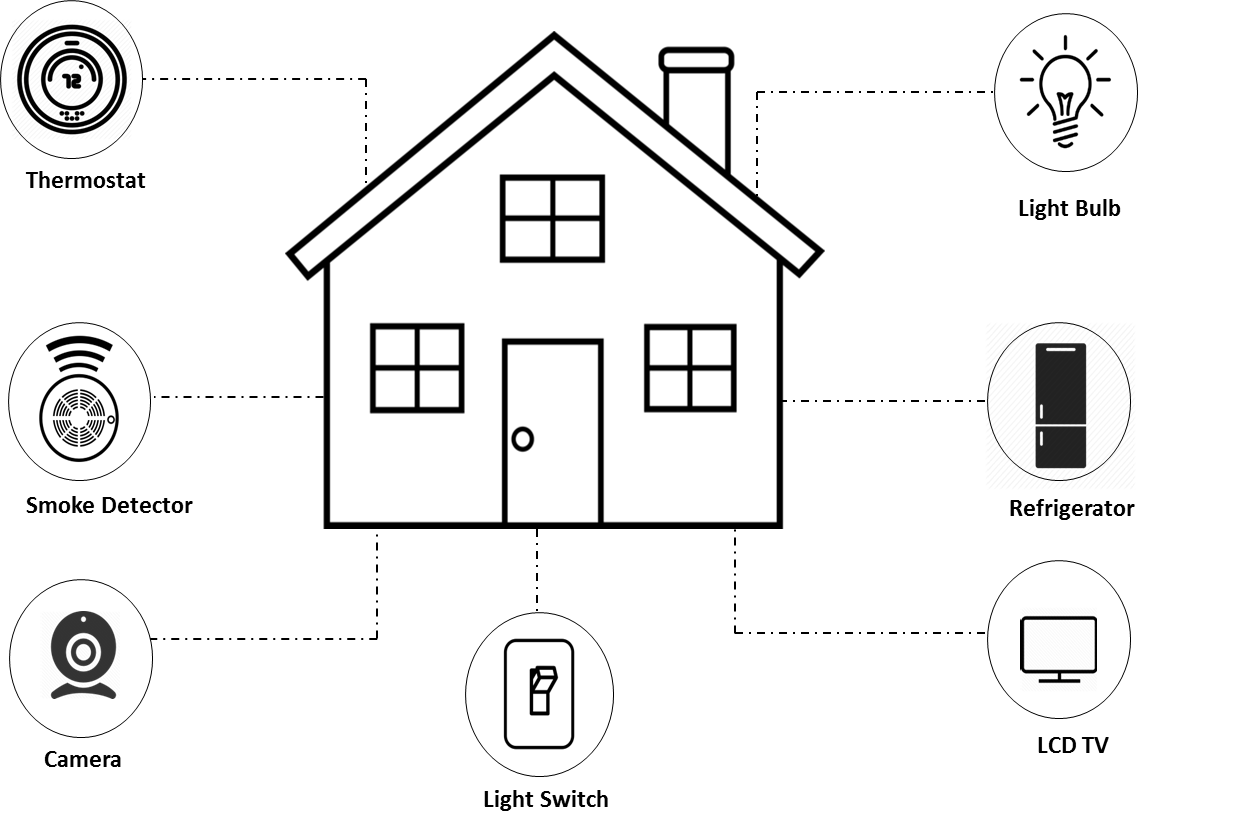
\includegraphics[height=3in]{smart_home_use_case.png}
%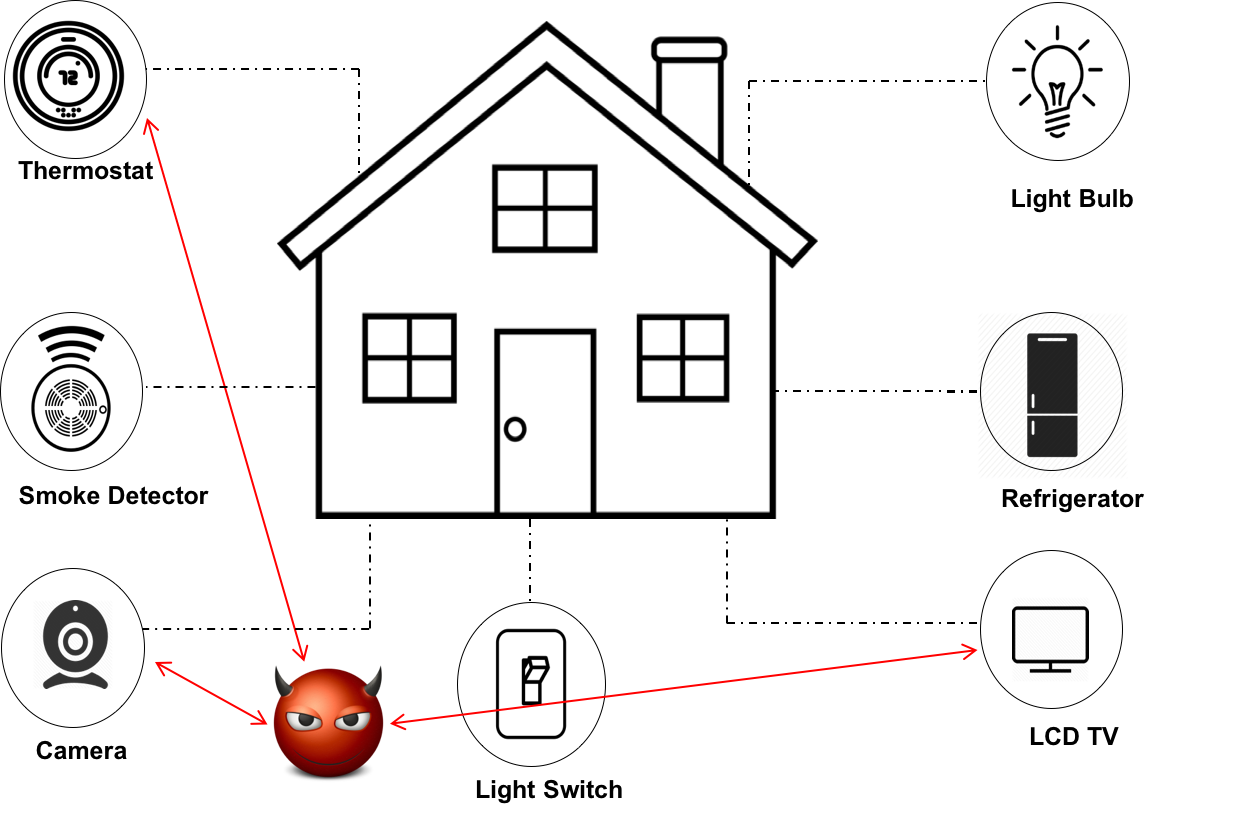
\includegraphics[height=4in]{smart_home_2.png}
%\end{center}
%\caption{Smart home use case Diagram}
%\label{smart_home}
%\end{figure}



%Consider a smart home as illustrated in Figure \ref{smart_home} that contains interconnected devices such as a thermostat which automatically detects and regulates the temperature of a room based on prior information of a user's temperature preferences, a smart lock system that can be controlled remotely and informs a user via short messaging when the door has been opened or is closed, a home security camera monitoring system, a smart fridge which sends a reminder when food products are low. In an event that a malicious intruder attempts  to gain access to the smart lock system and security camera remotely, provenance information can be used to track the series  of events to determine where and how a malicious attack originated. Provenance can also be used as a safeguard to alert of a possible remote or insider compromise thereby protecting against future or ongoing malicious attacks. 





%\section{Research Questions}
%The unification of data provenance and CPS and IoT is essential to the security of data disseminated. However, the unification raises some important research issues some of which are as a result of pre-existing provenance and IoT related issues. Some of the issues raised as a result of the unification of data provenance with IoT are outlined below:
%
%\begin{itemize}
%
%\item \textbf{Modeling provenance data:} How do we model provenance data collected from sensors and actuators contained in IoT architecture? Are there models used to represent causality between sensor and actuator readings in the IoT architecture.
%
%\item \textbf{Memory constraints on IoT Devices:} The vast amounts of data generated leads to high storage space utilization. Memory and data management techniques should be employed for efficient storage of provenance data on memory constrained devices. How do we effectively collect provenance data in resource constrained devices and relate this information across layers of the IoT architecture
%
%
%
%\item \textbf{Provenance data application utilization:} How do we utilize provenance data generated by provenance collection system to provide intrusion detection or digital forensics.
%
%
%
%\end{itemize}

\section{Research Contribution}

This dissertation makes the following contributions:


\begin{itemize}

\item \textbf{Prov-CPS: trace-based provenance collection framework.} The design and implementation of a provenance collection framework for capturing trace-based events for tracking data flow in an application's logic. This framework generates a trace of streaming events through application instrumentation with low execution run-time overhead that is decoupled from the more resource-intensive activities of provenance processing and analysis.

\item \textbf{Provenance data model for trace events.} A unified data model that represents the information flow semantics of data movement among components in an abstract CPS. This abstraction is mapped to real CPSs to facilitate automation of provenance data collection and analysis.

\item \textbf{Storage optimization through trace event pruning.} Support within the Prov-CPS framework for data pruning algorithms that discard events from streaming trace data prior to their conversion to provenance. These algorithms can be tailored to the needs of the provenance analyst yet take advantage of application domain knowledge.

\item \textbf{Experimental evaluation of Prov-CPS.} Evaluation of the efficiency of Prov-CPS in space, with and without pruning, using a provenance-based IDS that identifies anomalies in data provenance records.



\end{itemize}

\section{Organization of Dissertation}

The remaining portion of this dissertation is organized as follows: In chapter 2, we review background information on CPS, Anomaly detection, and data provenance. We also discusses PROV-DM, a provenance ontological construct. In Chapter 3, we outline related work on provenance collection systems, provenance-based pruning techniques, and provenance-based intrusion detection. In Chapter 4, we give a detailed description of Prov-CPS, and provenance-trace data model. In Chapter 5, we describe our pruning heuristics. In Chapter 6, we discuss our anomaly detection algorithm using provenance graphs. Finally, we conclude in Chapter 7 with future research directions.

         % Introductory Chapter
\chapter{Background}

In this chapter, we describe concepts such as anomaly detection and data provenance. 

%\section{Cyber-Physical Systems}
%CPS is the combination of computation and physical component 


%\section{Internet of Things (IoT)}
%There is no standard definition for IoT, however, researchers have tried to define the concept of connected ``things". The concept of IoT was proposed by Mark Weiser in the early 1990s \cite{Mattern} which represents a way in which the physical objects, ``things", can be connected to the digital world. Gubbi et al \cite{park_provenance-based_2012} defines the IoT as  an interconnection of sensing and actuating devices that allows data sharing across platforms through a centralized framework. We define (IoT) as follows:
%
%\begin{definition}
%The Internet of Things (IoT) is a network of heterogeneous devices with sensing and actuating capabilities communicating over the internet. 
%
%\end{definition}
%
%The notion of IoT has been attributed to smart devices. The interconnectivity between various heterogeneous devices allows for devices to share information in a unique manner. Analytics is a driving force for IoT. With analytics, devices can learn from user data to make smarter decisions. This notion of smart devices is seen in various commercial applications such as smartwatches, thermostats that automatically learns a user patterns. The ubiquitous nature of these devices make them ideal choices to be included in consumer products. IoT architecture consists of four distinct layers: The sensor and actuator layer, device layer, gateway layer and the cloud layer. 
%
%\par With the recent data explosion \cite{emc_bigdata} due to the large influx in amounts of interconnected devices, information is disseminated at a fast rate and with this increase involves security and privacy concerns. Creating a provenance-aware system is beneficial to IoT because it ensures the trust and  integrity of interconnected devices. Enabling provenance collection in IoT devices allows these devices to capture valuable information which enables backtracking in an event of a malicious attack. We take a holistic approach to provenance collection by looking at how provenance information is collected across an IoT architectural framework.

 
%  \subsection{IoT Architecture}
%
%IoT architecture represents a functional hierarchy of how information is disseminated across multiple hierarchies contained in an IoT framework; from devices which contain sensing and actuating capabilities to massive data centers (cloud storage). Knowing how information is transmitted across layers allows a better understanding on how to model the flow of information across actors contained in an IoT hierarchy. 
%\par Figure \ref{iot_architecture} displays the IoT architecture and the interactions between the respective  layers. The base of the architectural stack consist of sensors and actuators which gathers provenance information and interacts with the device layer. The device layer consists of devices (e.g mobile phones, laptops, smart devices) which are responsible for aggregating data collected from sensors and actuators. These devices in turn forwards the aggregated data to the gateway layer. The gateway layer routes and forwards data collected from the device later. It could also serve as a medium of temporary storage and data processing. The cloud layer is involved with the storage and processing of data collected from the gateway layer. Note that the resource constraints decreases up the architectural stack with the cloud layer having the most resources (memory, power computation) and the sensor-actuator layer having the least. 
%
%
%\begin{figure}[h]
%\begin{center}
%
%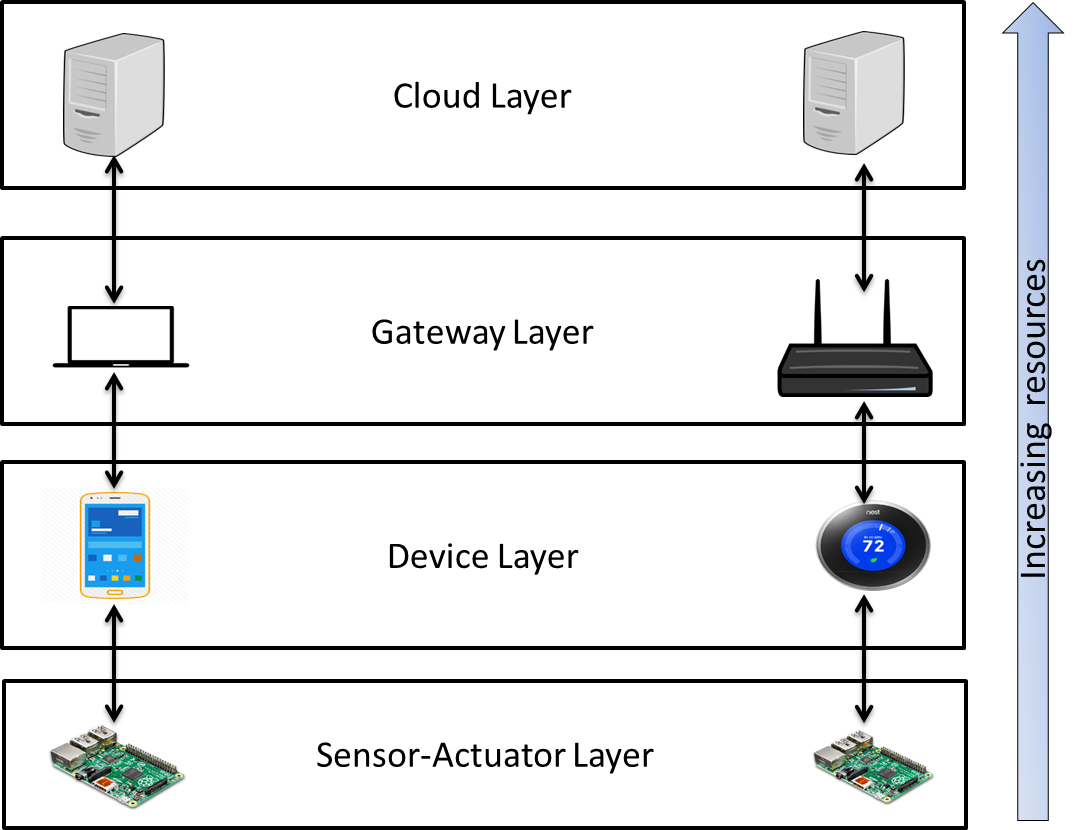
\includegraphics[height=3.0in]{iot_architecture.png}
%\end{center}
%\caption{IoT Architecture Diagram. The arrows illustrates the interaction between data at various layers on the architecture.}
%\label{iot_architecture}
%
%\end{figure}
%
%\section{Cyber- Physical System}


\subsection{Anomaly Detection}

The notion of what constitutes an anomaly is often domain specific. Hawkins defines an anomaly as an ``observation which deviates so much from the other observations as to arouse that it was generated by a different mechanism" \cite{hawkins}. In computing, an anomaly often indicates the presence of a malicious intrusion or a system fault. For example, an anomaly could be a sudden increase in web traffic of a web server which could be indicative of a denial of service attack. Additionally, in a critical care health device such as a pacemaker, an anomalous event could be detrimental to the health of a patient which could result in the loss of life. 

%Anomaly detection consists of two phase, learning phase also known as the training phase and the test also known as the detection phase. In the training phase, the system collects training dataset. This data is considered to be a representation of the system's normal daily activity and free from malicious events. Once training dataset has been collected, the system's activities are further observed. This part is known as the testing phase. In the testing phase,  observed system behavior is compared to the learning phase to determine is an anomaly exists between the two. A threshold as defined by domain experts is used to determine if the observed data is considered an anomaly.

%Data labels are grouped into three major categories. Supervised anomaly detection, semi-supervised anomaly detection, and unsupervised anomaly detection. In supervised anomaly detection approach, training data contains instances of normal and anomalous data. Incoming data is classified based on the training data category. In semi-supervised approach, only one class of training data is collected, normal data. Incoming data that does not fit the normal class as specified by a threshold is regarded as an anomalous. In the training phase, most anomaly detection techniques use data derived from the normal system behavior.  This is referred to as one class classification. In unsupervised approach, there are no training dataset. it is believed that normal data is clustered around each and occurs more frequently than an anomaly. This is a widely used form of anomaly detection since training data which is hard to get is not requited. 


Anomaly detection involves the use of rule-based, statistical, clustering or classification techniques to determine normal or anomalous data instances. The process of determining all anomalous instances in a given dataset or system is a complex task. A major challenge in anomaly detection is providing the right feature set from the data to use for detection. Another challenge exists in defining what constitutes as normal system behavior. Most anomaly detection using point based data often fail to include the dependencies that exist between data points.   

\section{Data Provenance}

Provenance is defined as ``The place of origin or earliest known history of something"~\cite{TCDP1999}. However, provenance and lineage are used interchangeably to denote the origin of something and transformation(s) that occurred to it over time. The notion of provenance originates from the art world, where an art piece auctioned is accompanied by a paper trail that denotes the artwork's chain of custody. This trail allows a buyer to ascertain the authenticity of the artwork. Likewise in computing, provenance provides a holistic history of data transformations that occur on a data object from inception to its present state. 

Data provenance can ensure data integrity \cite{Bertino2015} and establish causality between data objects through information-flow tracking.
Characteristic information provided by provenance include the who, where, when, and what of data transformation. \textbf{Who} identifies an actor responsible for a particular transformation of a data object. An example of ``who" in a CPS use case is a sensor, which is identified as the ultimate progenitor of values dervied from its sensor readings. \textbf{Where} provides the location of a transformation, for example a geolocation for the sensor. \textbf{When} associates time with a transformation, e.g., a timestamp obtained when a particular sensor reading was taken. \textbf{What} denotes the kind of transformation, such as a {\em read} operation or a {\em send} operation.

Provenance has been applied to database management to track the derivation of a query, in forensic analysis to determine what activities led to a system event~\cite{Bates2014LetSB, Lu:2010:SPE:1755688.1755723, 6542529}, in scientific experimentation for experiment reproducibility~\cite{chimera, Davidson:2008:PSW:1376616.1376772, altintas, Oinn2004TavernaAT}, and in intrusion detection~\cite{Xie_yulani, Fadolalkarim, 203308} to detect what activity might be responsible for a malicious compromise.

The increase in applications of provenance has led to provenance collection systems to support them. For example, within the context of the operating system, PASS~\cite{muniswamy_reddy} and HiFi~\cite{hi_fi} are two Linux-based provenance collection systems developed to capture interactions between files and system call events. In the scientific community, Chimera~\cite{chimera} and myGrid~\cite{Oinn2004TavernaAT} collect provenance to support scientific experiment workflow reproducibility. Notably, most of these applications are tailored for large-scale, memory-intensive applications that are difficult to adapt directly to memory-constrained CPS devices.





%The Oxford English dictionary defines provenance \cite{TCDP1999} as ``the place of origin or earliest known history of something". An example of provenance can be seen with a college transcript. A transcript is the provenance of a college degree because it outlines all of the courses satisfied in order to attain the degree.
%
%
%In the field of computing, data provenance, also known as  data lineage, can be defined as the history of all activities performed on entities from its creation to its current state. Cheney et al. \cite{cheney_provenance_2009} decribes provenance as the origin and history of data from its lifecycle. Buneman et al \cite{buneman_why_2001} describes provenance from a database perspective as the origin of data and the steps in which it is derived in the database system.  Provenance involves two granularity levels: fine-grained provenance and coarse-grained provenance. Fine-grained provenance \cite{glavic_case_2011} entails the collection of a detailed level of provenance. Coarse grained provenance, on the other hand, is a collection of a summarized version of provenance. Data provenance has immense applications and has been explored in the areas of scientific computing \cite{groth, altintas} to track how an experiments are produced, in business to determine the work-flow of  a process, and in computer security for forensic analysis and intrusion detection \cite{bates_towards_2013, muniswamy_reddy_provenance_2010, muniswamy_reddy} . 
%
%
%Provenance denotes the who, where and why of data \cite{cheney_provenance_2009}. An example of provenance for a software system is a web server's log file. This file contains metadata for various request and response time and the ip address of all host systems that requests information from the server. This log file identifies the data object (i.e. Web server), transformations that occurs on this object (e.g read write connections) and the state of the data object. Provenance data is represented as an acyclic graph which denotes casual relationship and dependencies between entities. 
%
%\par Provenance ensures trust and integrity of data \cite{Bertino2015}. It outlines causality and dependency between all objects involved in the system and allows for the verification of the source of data. Causality and dependency are used to determine the relationship between multiple objects. The relationship in which provenance denotes can in turn be used in digital forensics \cite{zawoadfecloud} to investigate the cause of a malicious attack and also in intrusion detection systems to further enhance the security of computing devices. 
% 
%
%Characteristic information provided by provenance include the who, where, when, and what of data transformation. \textbf{Who} identifies an actor responsible for a particular transformation of a data object. An example of ``who" in a CPS use case is a sensor, which is identified as the ultimate progenitor of values dervied from its sensor readings. \textbf{Where} provides the location of a transformation, for example a geolocation for the sensor. \textbf{When} associates time with a transformation, e.g., a timestamp obtained when a particular sensor reading was taken. \textbf{What} denotes the kind of transformation, such as a {\em read} operation or a {\em send} operation.

%\section{Comparing Provenance with Log Data and Metadata}
%
%Provenance data, log data and metadata are key data concepts that often are used interchangeably. We try to address the differences and similarities between provenance data, metadata and log data.
%
%\subsection{Provenance and Metadata}
%Metadata and provenance are often considered related but yet subtle distinctions exist. Metadata contains descriptive information about data. Metadata can be considered as provenance when there exists a relationship between objects and they explain the transformation that occurs. In summary,  metadata and provenance are not the same, however an overlap exists. Metadata contains valuable  provenance information but not all metadata is provenance information. 
%
%
%\subsection{Provenance and Log data}
%Log data contains information about the activities of an operating system or processes. Log data can be used as provenance because It contains data trace specific to an application domain. Log files might contain unrelated information such as error messages, warnings which might not be considered as provenance data. Provenance allows for specified collection of information that relates to the change of the internal state of an object. In summary, log data could provide insight to what provenance data to collect. 


 

%
%\section{IoT Application Use Case}

\section{Model for representing data provenance}

%In order to represent the right kind of provenance information, we need to satisfy the who, where, how, and what of data transformations. Provenance data can be represented using a provenance model in a modeling language such as, PROV\-DM which is represented in serialized form as a JSON object. This model displays the causal relationship of data objects. We propose a model that contains information such as sensor readings, device name, and device information. Details on the PROV-DM and PROV-JSON are outlined below.


To facilitate the creation of cross-platform provenance, an abstract representation of provenance typically uses a directed acyclic graph (DAG) in which vertices correspond to data and edges to interactions between data. A selection of vertex types and edge relationships constitutes a provenance model. The W3C standardizes a provenance ontology and a provenance data model, PROV-DM, to enable interchangeable provenance across heterogeneous systems. We adopt notions from the PROV-DM in the creation of Prov-CPS.


%We adopt the Provenance Data Model (PROV-DM) \cite{prov_dm}, a W3C standard which conforms to Provenance Ontology (PROV-O) and is used to depict dependencies between entities, activities and agents (digital or physical). PROV-DM creates a common model that allows for interchange of provenance information between heterogeneous devices and is represented serialized in three formats:  XML, JSON and RDF. 

\par PROV-DM contains two major components: types and relations.  Types can be entities, activities, or agents. An entity is a physical or digital object. An activity represents some form of action that occurs over time.  An agent takes ownership of an entity, or performs an activity. Figure \ref{prov_rep} illustrates the types and relations contained in PROV-DM and their graphical representation. Entities, activities and agents are represented as oval, rectangular and pentagonal shapes respectively. 


\begin{figure}[h!]
\begin{center}

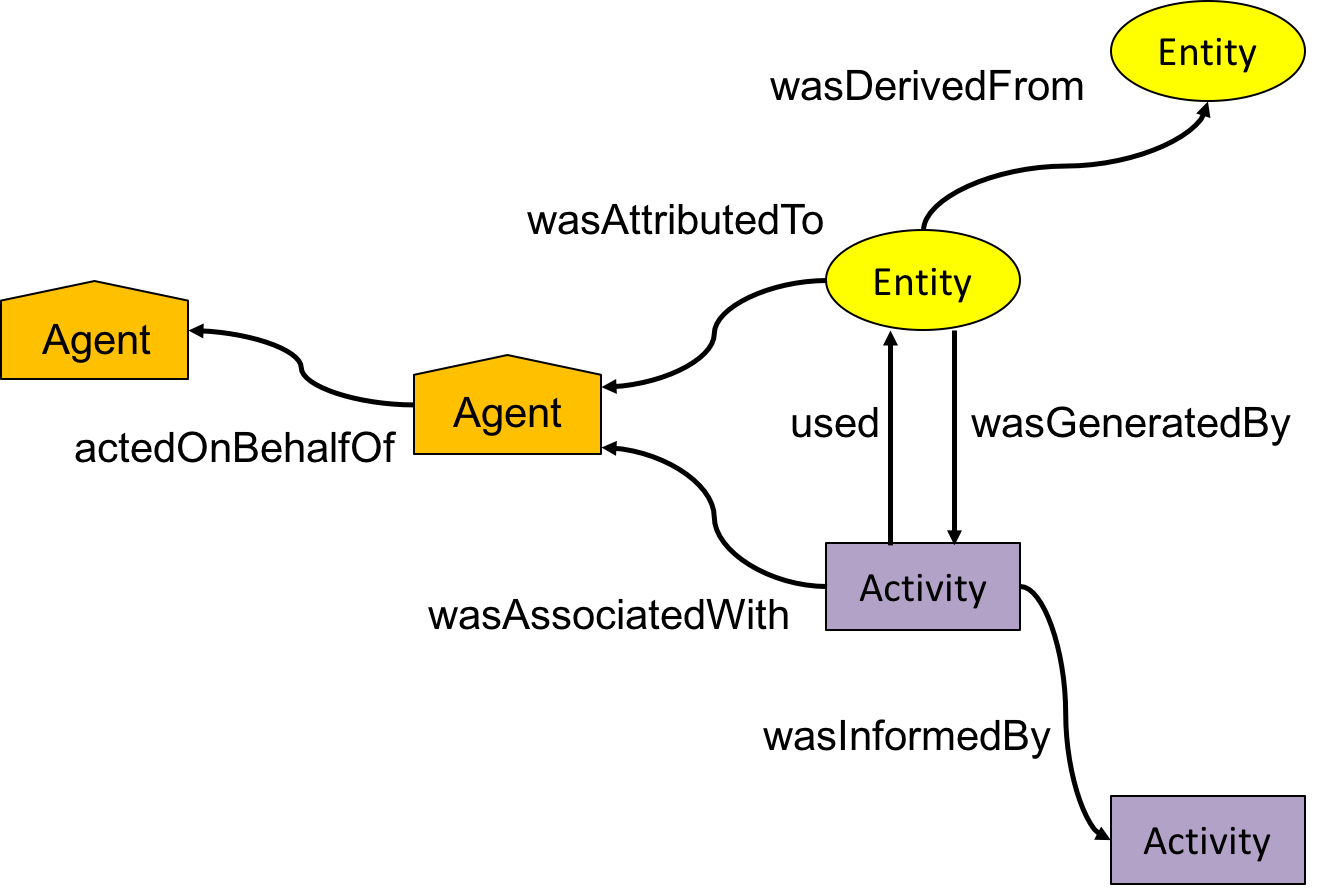
\includegraphics[width=0.7\textwidth]{prov_dm_2.PNG}
\end{center}
\caption{Prov-DM respresentation showing types in the model (Entity, Activity, and Agent) and the relationships between them }
\label{prov_rep}
\end{figure}


\par PROV-DM defines the following seven relationships between the types. 

\begin{itemize}
\item wasGeneratedBy: Signifies the production of a new entity by an activity. 

\item used: An entity generated by one activity has been adopted by another activity.

\item wasInformedBy: Signifies the exchange of an entity by two activities.

\item wasDerivedFrom: Represents a copy of information from an entity. 

\item wasAttributedTo: Denotes relational dependency between an entity and an agent when the activity that created the agent is unknown.

\item wasAssociatedWith: An agent created or modified the activity

\item actedOnBehalfOf: Delegation of authority from an agent to itself or another agent to perform a particular responsibility. 



\end{itemize}


Using the terminology of PROV-DM, we formally define a provenance graph as a labeled directed acyclic graph, $p = (V,E)$ where $V$ is a set of vertices $V =\{v_1,...,v_n\}$ such that $v_i = (type, value)$, with type one of the core types of PROV-DM, and $E$ is a set of edges $E =\{e_1,..., e_n\}$ where $e_i = (v_s, v_d, label)$, with $v_s, v_d$ as source and destination vertices, and $label$ is one of the PROV-DM relations. Two vertices $v_x$, $v_y$ are equal (denoted $ v_x = v_y$) if $v_x.type = v_y.type$ and $v_x.value = v_y.value$. Two edges $e_x $ and $e_y$ are equal (denoted $e_x = e_y$) if $e_x.v_s = e_y.v_s$, $e_x.v_d = e_y.v_d$, and $e_x.label = e_y.label$.  We use the union operator $\cup$ over edge sets in the usual way of the union of sets.



%
%\subsection{Provenance Data Model (Prov-DM)}
%
%Another model for representing provenance data is the Provenance Data Model (PROV\-DM). PROV-DM is a W3C standardized extension of OPM. Prov-DM is a model that is used to depict causal relationships between entities, activities and agents (digital or physical). It creates a common model that allows for interchange of provenance information between heterogeneous devices. It contains two major components: types and relations. 
%
%
%\begin{itemize}
%
%\item Entity: An entity is a physical or digital object. An example of an entity is a file system, a process, or an motor vehicle. An entity may be physical or abstract.
%
%\item Activity: An activity represents some form of action that occurs over a time frame. Actions are acted upon by an agent. An example of an activity is a process opening a file directory, Accessing a remote server.
%
%\item Agent: An agent is a thing that takes ownership of an entity, or performs an activity. An example of an agent is a person, a software product, or a process.
%\end{itemize}
%
%The figure below illustrates the various types contained in PROV-DM and their representation. Entities, activities and agents are represented by oval, rectangle and hexagonal shapes respectively.
%
%\begin{figure}[h]
%\begin{center}
%
%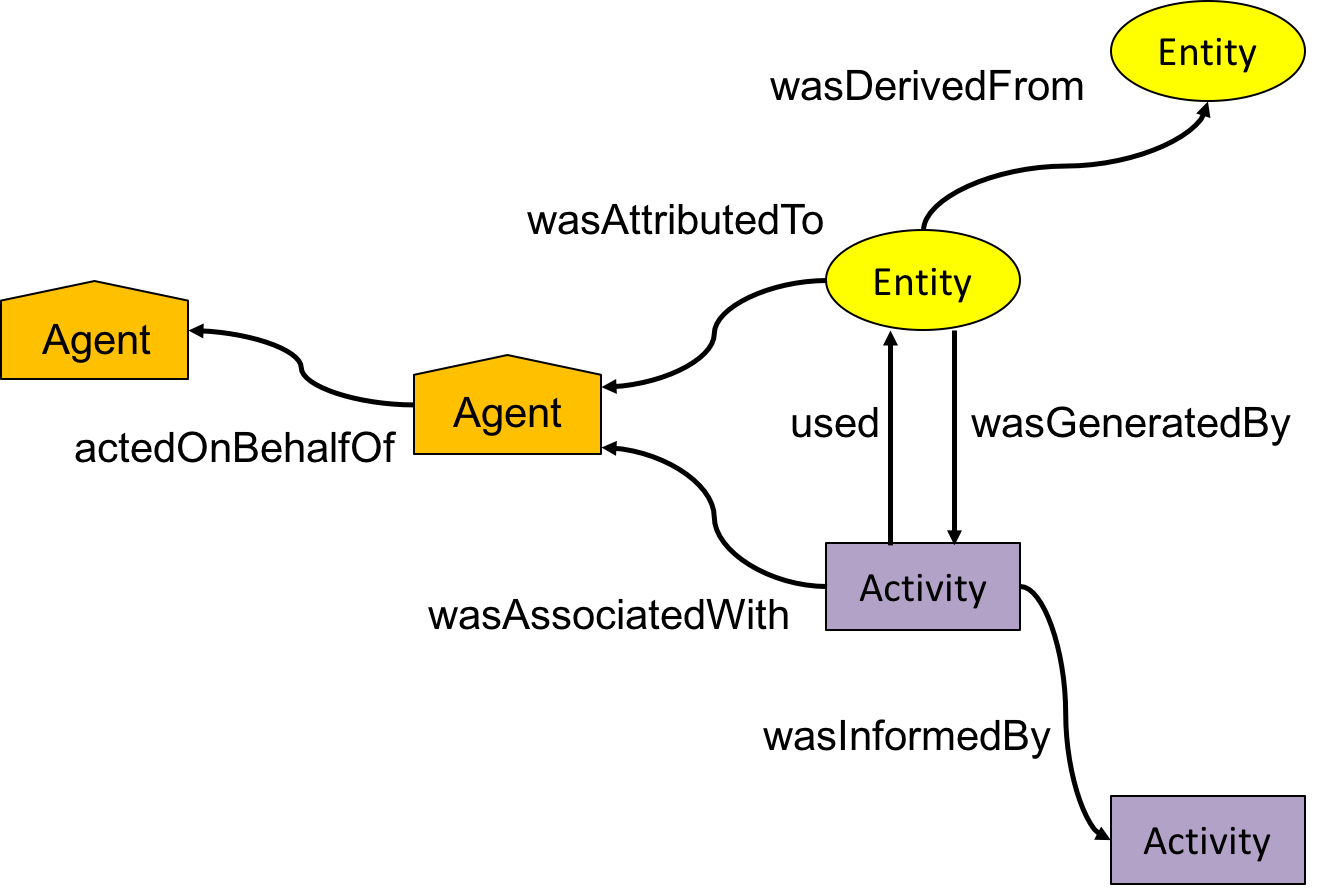
\includegraphics[width=4.0in]{prov_dm_2.PNG}
%\end{center}
%\caption{Prov-DM respresentation showing various types contained in the model (Entity, Activity, and Agent) }
%\end{figure}
%
%Similar to the OPM, PROV-DM does not keep track of future events. PROV-DM relations are outlined below:
%
%
%\begin{itemize}
%\item wasGeneratedBy: This relation signifies the creation of an entity by an activity. 
%
%\item used: This relation denotes that the functionality of an entity has been adopted by an activity.
%
%\item wasInformedBy: This relation denotes a causality that follows the exchange of two activities.
%
%\item wasDerivedFrom: This relation represents a copy of information from an entity. 
%
%\item wasAttributedTo: This denotes relational dependency to an agent. It is used to denote relationship between entity and agent when the activity that created the agent is unknown.
%
%\item wasAssociatedWith: This relation denotes a direct association to an agent for an activity that occurs. This indicates that an agent plays a role in the creation or modification of the activity.
%
%\item actedOnBehalfOf: This relation denotes assigning authority to perform a particular responsibility to an agent. This could be by itself or to another agent.
%
%
%
%\end{itemize}
%
%Some of the difference between OPM and PROV-DM are described below:
%
%\begin{itemize}
%
%\item The main components Artifact, Process and Agent in the OPM model are modified to Entity, Action, and Agent. 
%
%\item Additional causal dependencies such as wasAttributedTo and actedOnBehalfOf were included to represent direct and indirect causal dependencies respectively between agents and entities.
%
%\end{itemize}

%Since PROV-DM is built ontop of OPM and contains easy to understand constructs of types and relations. We are envision are properly represented through the various types and relations, we choose this model to represent provenance data in our IoT architecture instead of OPM. 

%\subsection{PROV-JSON}
%
%PROV-JSON is used for representing PROV-DM data in JSON (JavaScript Object Notation) format. It contains all of the components and relationships contained in PROV-DM and allows for easy serialization and deserialization. JSON is a lightweight data format which is human readable and easy to parse. Figure \ref{provjson} illustrates a use case for the serialization of PROV-DM to PROV-JSON. PROV-JSON contains key-value pairs and can be considered as an indexed version of PROV-DM. The example illustrates the relationship in which s1 tries to access a file (FileB) which was generated by s2. PROV-JSON  contains an entity, activity and agent type which are represented as a json objects and are identified by their respective ids.  Identifiers are optional in PROV-DM but are required for PROV-JSON since json objects contains key-value pairs, the id's of each object has to be implicitly specified and cannot contain null values. 
%
%\begin{figure}[h!]
%\begin{center}
%
%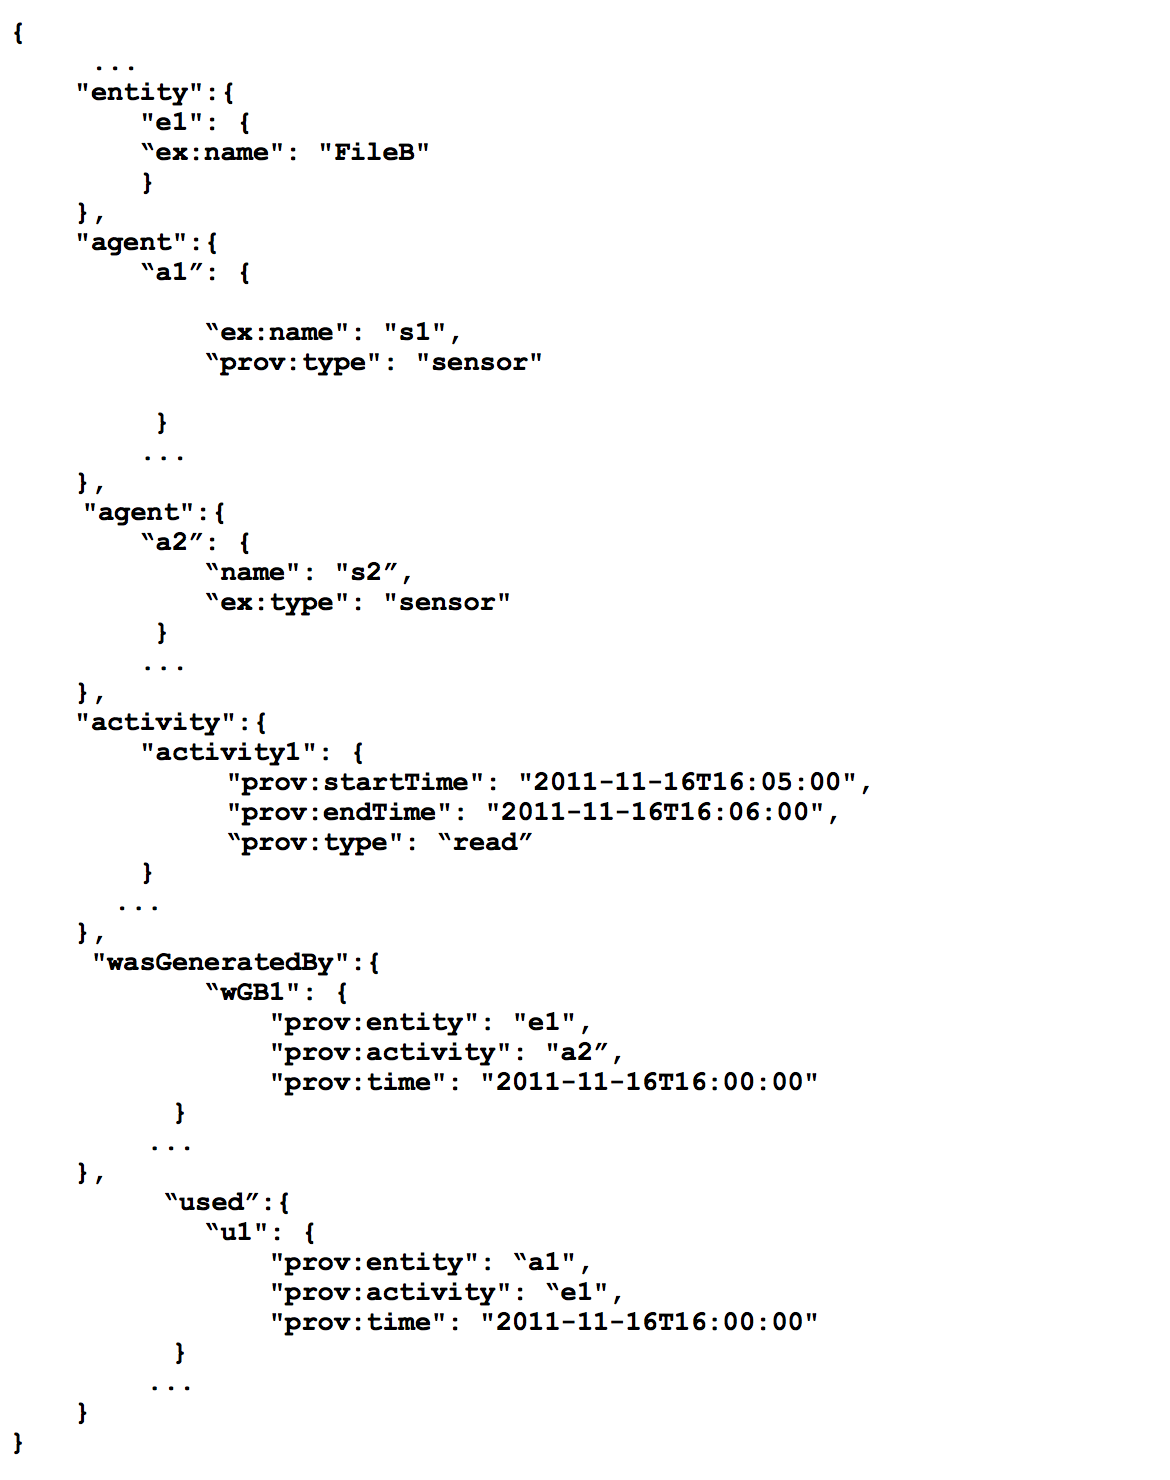
\includegraphics[height=5.7in]{prov_json_edit.png}
%\end{center}
%\caption{PROV-JSON MODEL \copyright \cite{prov_json}}
%
%\label{provjson}
%
%\end{figure}
%
%
%Each object contains fields which assigns additional attributes to the relations (i.e name, type, prov:startTime).  PROV-JSON documents might also contain a prefix object which defines namspaces that are used in the document. In this object is contained a default field which is used to define all of the namespace that contains all other unprefixed namespace.


%\subsection{Similarity Metric} \label{similarity}
%Similarity metric is a measure of how identical two objects are, for example, by measuring the angle between objects (using cosine similarity) or a linear distance (using euclidean distance) between the objects. In this work, we use cosine similarity as our similarity metric. Cosine similarity is a measure of orientation between two non-zero vectors. It measures the cosine of the angle between the vectors. Two vectors which are at an angle of 90\degree  have a similarity of 0, two vectors which are identical (with an angle of 0\degree) have a cosine of 1, and two vectors which are completely opposite (with an angle of 180\degree) have a similarity of -1. Since we are concerned with the similarity of the vectors, we are only concerned with the positive values bounded in [0,1]. To compute the cosine similarity between two vectors, $X$ and $Y$:
%
%\[\mathbf{\cos{(\theta)}} = \dfrac{X \cdot  Y}{ \lVert \mathbf{X} \rVert \cdot \lVert \mathbf{Y} \rVert} =\dfrac{\sum_{i}^n X_i Y_i }{\sqrt[]{\sum_{i}^n X_i^2} \sqrt[]{\sum_{i}^n Y_i^2}}  \]
%
%\subsubsection{Jaccard Similarity}
%This similarity measure evaluates the intersection divided by the union of two non zero vectors.
%
%\[ J(X,Y) = \dfrac{|X \cap Y | }{| X \cup Y |} \]
%
%\subsubsection{Euclidean distance}
%This measures calculates the line distance between two data objects in an euclidean space. The euclidean distance between vectors $X$ and $Y$ , $d(X, Y)$ is defined by: 
%
%\[ d(X, Y) =  \sqrt{\sum_{i=1}^n (X_i - Y_i)^2} \]




%\subsection{A Review of Machine Learning Techniques: $DBSCAN$ and $k$-nearest neighbors}
%
%\subsubsection{$k$-Nearest Neighbors:} $k$-NN is an instance based supervised learning algorithm for data classification. Data is grouped on its similarity to nearest neighbors where $k$ denotes the number of neighbors in which the input data is compared to.  A similarity measure such as euclidean distance, jaccard similarity, or cosine similarity is used to measure the distance between vectors. $k$-NN can be applied to classification and regression problems.
%
%Researchers have proposed various modifications to the $k$-NN algorithm. Ramaswamy et al. \cite{Ramaswamy} proposed a $k$-NN modification which calculates the sparseness estimates for vectors in a dataset. The vectors are sorted in increasing order according the distance from its $k^{th}$ neighbor. Bay and Swabacher demonstrates how pruning irrelevant datapoint which are not considered anomalous can result in a linear complexity of nearest neighbor search for a randomized data. A threshold score is assigned which is based on the score of the weakest anomaly found. Pruning can be achieved by using the  relative density of data points, an anomaly is believed to occur in a group of data points with low density.
%
%\subsubsection{Density Based Spatial Clustering of Applications with Noise ($DBSCAN$):}
%
%\textit{DBSCAN} is a density-based clustering algorithm that differentiates regions with high density from regions with low density. It defines two parameters $\boldsymbol{\varepsilon}$, and $\boldsymbol{MinPts}$. $\varepsilon$ defines the maximum distance between two neighboring points in which they are considered to be in the same cluster. $MinPts$ is the minimum number of points that can be contained in a cluster. 
%
%Let $S = \{s_1, s_2,...s_n \}$ be a set of point to be clustered. $S$ consists of three point categories, a core point, $\boldsymbol{q}$, a border point, $b$ and a noise point, $n$. A core point is a point in which its $minPts$ are within distance $\varepsilon$. These are at the interior of the cluster. Border points are points on the edge of the cluster. A noise point (outlier) is any point that is neither a core point or a border point. A point, $l$ is directly reachable from a core point, $q$ if there exist a path which is within distance of $\varepsilon$ from the core another point. (i.e $ \exists \quad  \{q_1, q_2,...q_n \}, \textrm{where} \quad |q_{i+1}  - q_i| \leq \varepsilon$ ). A core point, $\boldsymbol{q}$ that is within distance $\varepsilon$ (i.e $q \leq \varepsilon$) is considered part of the same cluster. A border point is also considered part of a cluster if it close to a core point. A cluster consists of at least one core point.
%
%
%%\subsubsection{ $k$ means clustering:}



%\subsection{Provenance Graph to Vector Space Conversion }







%\section{Policy Model}
%
%\subsection{eXtensible Access Control Markup Language (XACML)}
% XACML is an access control policy language that allows the creation and enforcement of policies written in XML. It is a standard specification developed by the Organization of Advancement of Structured Information Standards (OASIS). Since it is written in XML, this framework allows for extensible and flexible policy documents. XACML consists of three major components which are involved in policy generation, evaluation and enforcement. The components of XACML are described below: 
% 
% 
% \begin{itemize}
% 
% \item Policy Administration Point (PAP): This component of XACML
%is involved with the generation of policy documents. A Policy document is created by specifications and requirements set aside by an administrator.
%
% \item Policy Decision Point (PDP): The Policy Decision Point evaluates policies by the request context generated by a user. Based on the request, It generates a response (accept,deny or intermediate) This response is communicated with the Policy Enforcement Point which enforces the response sent by the PDP.
%
%
%\item Policy Enforcement Point (PEP):  The Policy Enforcement Point generates request context which is sent to the PDP for evaluation. It is also involved with the responsibility of enforcing request based on decision received by the PDP.
%
% \end{itemize}
% 
% 
% 
% \begin{figure}[tbh]
%\begin{center}
%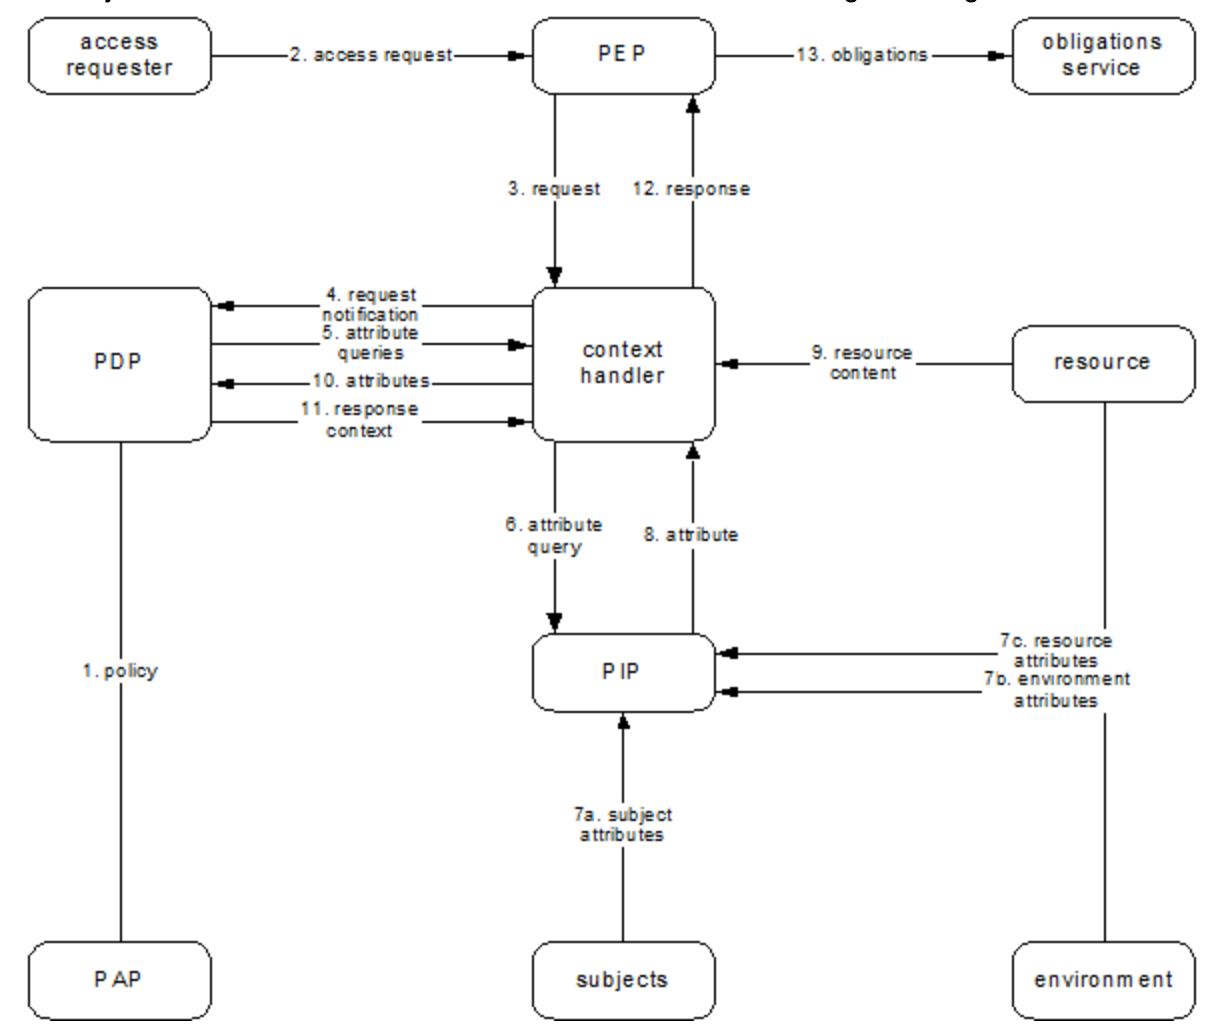
\includegraphics[height=3.5in]{xacml.png}
%\caption{Xacml Data-flow diagram  \copyright \cite{xacml}}
%\end{center}
%\end{figure}
 
%\section{Overview of Relevant Compression techniques}
%
%\subsection{Lossy Compression}
%
%Lossy compression \cite{Sayood:2000:IDC:336428} is a form of data compression in which original data can be reconstructed with some tolerance on loosing some information contained in the original data. This enables higher compression ratio than other compression techniques. Lossy Compression is mostly used in applications that do not contain strict requirements as to loosing some information. An example of a lossless compression application can be seen in an image compression software where the quality of the image is not seen by the naked eye. It is also used in speech transmission. 
%
%\subsection{Lossless Compression}
%Lossless compression \cite{Sayood:2000:IDC:336428} is a data compression technique in which the original data is reconstructed without loss of any information. It can be used by applications which requires that the data is compressed and the original data be identical. An example of such an application that requires lossless compression is text compression.  Any compression that alters the structure of the original text results to a different meaning of the text. For instance, the sentence ``I have a black cat" would have a different meaning if any information is lost from it.
%
%
%
%\subsubsection{Arithmetic Coding}
%
%Arithmetic coding is a form of lossless compression which encodes a stream of characters into a variable size interval between [0,1). A probability is assigned to each characters contained in the string. A cumulative probability is used to calculate the interval of the respective character. Frequent characters are encoded with shorter codes than less frequent characters. 


%\subsection{Anomaly Detection}
%
%The notion of what constitutes an anomaly is often domain specific. Hawkins defines an anomaly as an ``observation which deviates so much from the other observations as to arouse that it was generated by a different mechanism" \cite{hawkins}. In computing, an anomaly often indicates the presence of a malicious intrusion or a system fault. For example, an anomaly could be a sudden increase in web traffic of a web server which could be indicative of a denial of service attack. Additionally, in a critical care health device such as a pacemaker, an anomalous event could be detrimental to the health of a patient which could result in the loss of life. 
%
%Anomaly detection consists of two phase, learning phase also known as the training phase and the test also known as the detection phase. In the training phase, the system collects training dataset. This data is considered to be a representation of the system's normal daily activity and free from malicious events. Once training dataset has been collected, the system's activities are further observed. This part is known as the testing phase. In the testing phase,  observed system behavior is compared to the learning phase to determine is an anomaly exists between the two. A threshold as defined by domain experts is used to determine if the observed data is considered an anomaly.
%
%Data labels are grouped into three major categories. Supervised anomaly detection, semi-supervised anomaly detection, and unsupervised anomaly detection. In supervised anomaly detection approach, training data contains instances of normal and anomalous data. Incoming data is classified based on the training data category. In semi-supervised approach, only one class of training data is collected, normal data. Incoming data that does not fit the normal class as specified by a threshold is regarded as an anomalous. In the training phase, most anomaly detection techniques use data derived from the normal system behavior.  This is referred to as one class classification. In unsupervised approach, there are no training dataset. it is believed that normal data is clustered around each and occurs more frequently than an anomaly. This is a widely used form of anomaly detection since training data which is hard to get is not requited. 
%
%
%Anomaly detection involves the use of rule-based, statistical, clustering or classification techniques to determine normal or anomalous data instances. The process of determining all anomalous instances in a given dataset or system is a complex task. A major challenge in anomaly detection is providing the right feature set from the data to use for detection. Another challenge exists in defining what constitutes as normal system behavior. Most anomaly detection using point based data often fail to include the dependencies that exist between data points. 




%Graphs offers a means of modeling complex structures such as social networks, computer networks, biological DNA sequences.  




%Details on anomaly detection techniques are outlined below
%
%
%\begin{enumerate}[]
%
%
%\item Statistical-based approach: This approach involves the use of parametric or non parametric statistical inference to develop models which are used to determine if a dataset fits a statistical model. Instances that do not fit the defined statistical model are classified as an anomaly. 
%
%\item Classification: The main idea in this approach involves building models which use training data set with predefined labels (i.e normal, anomalous) to classify incoming data. Classification works in two phase: training phase and observation phase. In the training phase, data is collected which contains labels of normal and anomalous system behavior. If the dataset only contains a label of either anomalous or normal behavior, this is considered as a one class classifier. In the observation phase, incoming data is classified by defined data labels.
%\begin{itemize}
%
%\item Nearest-Neighbor: It is based on the assumption that normal data occurs in dense neighborhoods and abnormal data in sparse neighborhoods. The main idea is to assign an incoming observation data to a class based on its proximity to the closest data point in the training data set. A distance or similarity measure is used to quantify the distance between points in a dataset.  A popular form of nearest neighbor technique is the $k$-nearest neighbor which groups incoming data based on proximity to $k$ closest data point. Details on $k$- nearest neighbors is discussed in section 3.5. 
%
%\end{itemize}
%
%\item Clustering: The main idea is to group similar data instances into clusters. There are various approach to clustering. One approach looks at the density of the clusters, normal data belongs to large dense clusters while abnormal data belongs to small clusters. Another approach as treats clustering as one class which assumes that normal belongs to a cluster and abnormal data does not. Another approach looks at the distance of the data to the centroid. Centroids are seen as the center of the cluster. Normal data are  considered to be closer to the centroid than anomalies lie.
%
%\begin{itemize}
%
%\item Density: This approach is used to estimate the density of  $k$ nearest neighbors. A data instance in a dense neighborhood is considered normal while data instances in neighborhoods with a sparse density are considered anomalous. The distance from a data instance to a nearest neighbor is seen as the inverse of the density of data instances.  This approach faces an issue in which the density approach performs poorly in regions of varying densities. Local outlier factor addresses this issue. Local outlier factor is a measure of the degree of Outlieriness of each data instance contained in a data set. It is achieved by comparing the ratio of local density of k nearest neighbors to the density of a data instance. Data instances with lower density are considered outliers.
%
%\end{itemize}
%
%
%
%
%
%
%\end{enumerate}  




% chap2.tex (Definitions)



\chapter{Literature Review}\label{background}

This section discusses the state of the art in data provenance collection systems, pruning techniques for data provenance, and provenance-based intrusion detection systems.


\section{Data Provenance Collection Systems}

There has been a considerable amount of work done on data provenance collection \cite{_general-purpose_2012, bates_trustworthy_2015, gessiou_towards_2012, muniswamy_reddy_provenance_2010}. Some of the work done has been focused on databases, sensor networks, scientific workflow systems and file system provenance but so far little attention has been given to provenance in CPS. Some of the prior work done on data provenance collection are outlined as follows:



%System call provenance collection is further divided into kernel space provenance collection and user space provenance collection. Kernel involves provenance collection of system events such as files and system call. User space on the other

\subsubsection{Kernel space provenance collection}

Muniswamy-Reddy
et al. \cite{muniswamy_reddy} developed PASS, a provenance collection system that tracks  system-level provenance of the Linux file system. Provenance information
is stored in the same location as the file system for easy accessibility, backup,
restoration, and data management. Provenance information is collected and stored in
the kernel space. PASS is composed of 3 major components: provenance collector, provenance storage, and provenance query. The collector keeps track of system level provenance. It intercepts system calls which are translated into provenance data and initially stored in memory as inode cache. Provenance data is then transferred to a file system in an kernel database, BerkleyDB. This database maps key value pairs for provenance data for fast index look up. PASS collects and stores provenance information containing a reference to the executable that created the provenance data, input files, a description of hardware in which provenance data is produced, OS information, process environment, process parameters, and other data such as a random number generator seed. PASS detects and eliminates cycles that might occur in provenance dependencies as a result of version avoidance. Cycles violate the dependency relationships between entities. For example, a child node could depend on a parent node and also be an ancestor of a parent node. PASS eliminates cycles by merging processes that might have led to the cycles. It also provides functionality for querying provenance data in the database. The query tool is built on top of BerkleyDB. For querying provenance, users can process queries using the provenance explorer. Query is done using commands such as MAKEFILE  GENERATION which creates the sequence of events that led to the final state of a file or process. DUMP ALL, gets the provenance of the requested file. Our approach addresses application level provenance
for memory constrained embedded systems without requiring OS modification.


Pohly et al. \cite{hi_fi}  developed Hi-Fi, a system level provenance collection framework for the Linux kernel using Linux Provenance Modules (LPM), this framework tracks system level provenance such as interprocess communication, networking, and kernel activities. This is achieved by mediating access to kernel objects using Linux Security Model (LSM) which is a framework that was designed for providing custom access control into the Linux kernel. It consists of a set of hooks which executed before access decision is made. LSM was designed to avoid problem created by direct system call interception. The provenance information collected from the kernel space is securely transmitted to the provenance recorder in the user space. 
\par HiFi contains three components: provenance collector, provenance log and provenance handler. The collector and log are contained in the kernel space while the handler is contained in the user space. The log is a storage medium which transmits the provenance data to the user space. The collector uses LSM which resides in the kernel space. The collector records provenance data and writes it to the provenance log. The handler reads the provenance record from the log. This approach to collecting provenance data differs from our work since we focus on embedded systems and are concerned with input and output (I/O) data, which involves sensor and actuator readings. Additionally,  HiFi deals with collecting system level events which might incur additional overhead when compared to collecting application level provenance. HiFi is engineered to work solely on the Linux operating system. Embedded systems that do not run on Linux OS will not be able to incorporate HiFi. 

Bates et al \cite{bates_towards_2013} provide a security model for provenance collection in the linux kernel. This is achieved by creating a Linux Provenance Model (LPM). LPM serves as a security layer which provides a security abstraction for provenance data. It is involved in the attestation disclosure of the application layer and authentication channel for the network layer. The goal of LPM is to provide an end to end provenance capture system. LPM ensures the following security guarantees: For LPM, the system must be able to detect and avoid malicious forgery of provenance data. The system must be trusted and easily verifiable. \par When an application invokes a system call, the LPM tracks system level provenance which is transmitted to the provenance module via a buffer. The provenance module registers contain hooks which records system call events. These events are sent to a provenance recorder in the user space. The provenance recorder ensures that the provenance data is stored in the appropriate backend of choice. Provenance recorders offer storage support for Gzip, PostGreSQL, Neo4j and SNAP.

King and Chen \cite{King:2003:BI:945445.945467} developed a system, Backtracker, which generates an information flow of OS objects (e.g file, process) and events (e.g system call) in a computer system for the purpose of intrusion detection. From a detection point, information can be traced to pinpoint where a malicious attack occurred. The information flow represents a dependency graph which illustrates the relationship between system events. Detection point is a point in which an intrusion was discovered. Time is included in the dependency between objects to reduce false dependencies. Time is denoted by an increasing counter. The time is recorded as the difference of when a system call is invoked till when it ends. Backtracker is composed of two major components: EventLogger and GraphGen. An EventLogger is responsible for generating system level event log for applications running on the system. EventLogger is implemented in two ways: using a virtual machine and also as a stand alone system. In a virtual machine, the application and OS is run within a virtual machine. The OS running inside of the virtual machine is known as the guest OS while the OS on the bare-metal machine is known as the host OS, hypervisor or virtual machine monitor. The virtual machine alerts the EventLogger in the event that an application makes a system call and or exits. EventLogger gets event information, object identities, dependency relationship between events from the virtual machine's monitor and also the virtual machine's physical memory. EventLogger stores the collected information as a compressed file. EventLogger can also be implemented as a stand alone system which is incorporated in an operating system. Virtual machine is preferred to a standalone system because of the use of virtual machine allows ReVirt to be leveraged. ReVirt enables the replay of instruction by instruction execution of virtual machines. This allows for whole information capture of workloads. After the information has been captured by the EventLogger, GraphGen is used to produce visualizations that outlines the dependencies between events and objects contained in the system. GraphGen also allows for pruning of data using regular expressions which are used to filter the dependency graph and prioritize important portions of the dependency graph.





\subsubsection{User-space provenance collection}
RecProv \cite{rec_prov} is a provenance system which records user-level provenance, avoiding the overhead incurred by kernel level provenance recording. It does not require changes to the kernel like most provenance monitoring systems. It uses Mozilla rr to perform deterministic record and replay by monitoring system calls  and non deterministic input. Mozilla rr is a debugging tool for Linux browser. It is developed for the deterministic recording and replaying of the Firefox browser in Linux. RecProv uses PTRACE\_PEEKDATA from ptrace to access the dereferenced address of the traced process from the registers. Mozilla rr relies on ptrace, which intercepts system calls to monitor the CPU state during and after a system call. It ptrace to access the dereferenced address of the traced process from the registers. System calls are monitored for file versioning. The provenance information generated is converted into PROV-JSON, and stored in Neo4j, a graph database for visualization and storage of provenance graphs. Our approach
focuses on event flow of application logic on memory constrained CPS devices without requiring OS level interference.


Spillance et al \cite{story} developed a user space provenance collection system, Storybook, which allows for the collection of provenance data from the user space thereby reducing performance overhead. This system takes a modular approach that allows the use of application specific extensions allowing additions such as database provenance, system provenance, and web and email servers. It achieves provenance capture intercepting system level events on FUSE, a file system and MySQL , a relational database. StoryBook allows developers to implement provenance inspectors these are custom provenance models which captures the provenance of specific applications which are often modified by different application(e.g web servers, databases). When an operation is performed on a data object, the appropriate provenance model is triggered and provenance data for that data object is captured. StoryBook stores provenance information such as open, close, read or write, application specific provenance, and causality relationship between entities contained in the provenance system. Provenance data is stored in key value pairs using Stasis and Berkeley DB as the storage backend. It also allows the use of interoperable data specifications such as RDF to transfer data between various applications. Storybook allows for provenance query by looking up an inode in the ino hashtable. In our approach
to provenance collection, we are particularly interested in the
provenance collection of application event logic on memory constrained CPS devices.

Goshal et al \cite{ghoshal_provenance_2013} developed a framework for collecting provenance data from log files. They argue that log data contains vital information about a system and can be an important source of provenance information. Provenance is categorized based on two types: process provenance and data provenance. Process provenance involves collecting provenance information of the process in which provenance is captured. Data provenance on the other hand describes the history of data involved in the execution of a process. Provenance is collected by using a rule based approach which consists of a set of rules defined in XML. The framework consists of three major components. The rule engine which contains XML specifications for selecting, linking and remapping provenance objects from log files. The rule engine processes raw log files to structured provenance. There are three categories of rules as specified by the grammar. The match-set rules which selects provenance data based on a set of matching rules. Link rules which specifies relationship between provenance events and remap rules are used to specify an alias for a provenance object. The rule engine is integrated with the log processor. The log processor component is involved with parsing log files with information contained in the rule engine. It converts every matching log information to a provenance graph representing entities (vertices) and their relationship (edges). The adapter converts the structured provenance generated by the log processor into serialized XML format which is compatible with Karma, a provenance service application that is employed for the storage and querying of the provenance data collected.

\subsection{Provenance of Sensor Networks}
Lim et al. \cite{lim} developed a
model for calculating the trust of nodes contained in a sensor network by using data
provenance and data similarity as deciding factors to calculate trust. The value of
provenance signifies that the more similar a data value is, the higher the trust score.
Also, the more the provenance of similar values differ, the higher their trust score. The trust score of a system is affected by the trust score of the sensor that forwards data to the system. Provenance is determined by the path in which data travels through the sensor network. This work differs from our approach since the authors focus on creating a trust score
of nodes connected in a sensor network using data provenance and do not emphasize
how the provenance data is collected. We are focused on creating a
provenance aware system for application based events which are used to ensure trust of
connected devices. 

\subsection{Provenance collection on scientific experiments}
\par PReServ was developed to address the needs of specific application domain (Scientific experiments). It deals with recording process documentation of Service Oriented Architecture (SOA) and collects P-assertions which are assertions made about the execution (i.e., messages sent and received, state information) of actions by actors. The provenance collected by PReServ does not demonstrate causality and dependency between objects. In other words, the provenance data collected are not represented using a provenance model (e.g PROV-DM) that depicts causal relationship between provenance data. 

\subsection{Application Instrumentation-based provenance collection}
Grouth et al \cite{groth} developed a provenance collection system, PReServ which allows software developers to integrate provenance recording into their applications. They introduce P-assertion recording protocol as a way of monitoring process  documentation for Service Oriented Architecture (SOA) in the standard for grid systems. PReServ is the implementation of P-assertion recording protocol (PreP). PreP specifies how provenance can be recorded. PReServ contains a provenance store web service for recording and querying of P-assertions. P-assertions are provenance data generated by actors about the application execution. It contains information about the messages sent and received as well as state of the message. PReServ is composed of three layers, the message translator which is involved with converting all messages received via HTTP requests to XML format for the provenance store layer. The message translator also determines which plug-in handle to route incoming request to, the  Plug-Ins layer. It implements functionality that the Provenance Store component provides. This component allows third party developers to add new functionality to store provenance data without going through details of the code implementation. The backend component stores the P-assertions. Various backend implementations could be attached to the system by the plug-in component.

Tariq et al. \cite{tariq_towards_2012} developed a provenance collection system which automatically collects interprocess provenance of applications source code at run time. This takes a different approach from system level provenance capture. It achieves provenance capture by using LLVM compiler framework and SPADE provenance management system. LLVM is a framework that allows dynamic compilation techniques of applications written in C, C++, Objective-C, and Java. Provenance data is collected from function entry and exit calls and is inserted during compilation. LLVM contains an LLVM reporter. This is a Java class that parses the output file collected from the LLVM reporter and forwards the provenance data collected to the SPADE tracer. SPADE is a provenance management tool that allows for the transformation of domain specific activity in provenance data. The LLVM Tracer module tracks provenance at the exit and entry of each function. The output is an Open Provenance Model in which functions are represented by an OPM process, arguments and return values are represented as an OPM artifact. To minimize provenance record, users are allowed to specify what functions they would like to collect provenance information at run time. The LLVM optimizer generates a graph of the target application. This graph is used to perform reverse reachability analysis  from the functions contained in the graph. A workflow of how the framework works in collecting provenance is as follows:

\begin{itemize}
\item The application is compiled and converted into bitcode using the LLVM C compiler, clang.

\item The LLVM Tracer module is compiled as a library.

\item LLVM is run in combination with the Tracer, passed to include provenance data. 

\item Instrumentation bitcode is converted into assembly code via the compiler llc

%\item The socket code is compiled into assembly code.


\item  The instrumented application and assembly code is linked into an executable binary and sent to the SPADE kernel.
\end{itemize}


%One major limitation to this approach of collecting application level provenance is that a user is required to have the source code of the specific application in which provenance data is required. Also, provenance collection is limited to function's exit and entry points. Provenance collection deals with data pruning by allowing a user to specify what provenance data to collect which is similar to our policy based approach for efficient provenance data storage.


Gessiou et al \cite{gessiou_towards_2012} propose a dynamic instrumentation framework for data provenance collection that is universal and does not incur the overhead of kernel or source code modifications. This is achieved by using DTrace, a dynamic instrumentation utility that allows for the instrumentation of user-level and kernel-level code and with no overhead cost when disabled. The goal is to provide an easy extension to add provenance collection on any application regardless of its size or complexity. Provenance collection is implemented on the file system using PASS and evaluated on a database (SQLite) and a web browser (Safari). 
The logging component monitors all system calls for processes involved. The logging component contains information such as system-call arguments, return value, user id, process name, and timestamp. The logging components includes functionalities to collect library and functional calls. The authors argue that applying data provenance to different layers of the software stack can provide varying levels of information. Provenance needs to be captured at the layer in which it is closest to the information that is needed to be captured. Provenance information that pertains to complex system activities such as a web browser or a database are collected. The information is collected from a process system-call and functional-call based on valid entry points contained in the process. DTrace dynamic instrumentation helps in discovering interesting paths in a system in which data propagates. This helps users use this information to collect a more accurate provenance data.


ProvThings~\cite{Wang2017FearAL}, an IoT based provenance-collection framework and API, allows application developers to generate provenance through instrumentation of devices by identifying security sources and sinks through a selective instrumentation algorithm. This framework's implementation is focused on a Samsung-based IoT platform, SmartThings. ProvThings utilizes a policy-based approach to intrusion detection in which a provenance graph pattern is matched based on defined system behavior. One distinct difference between this approach and our is that ProvThings is focused on cloud-based devices connected to a hub. Our approach is based on provenance data collection pertaining to devices which might not be internet enabled.

ContextIoT~\cite{jia2017contexiot} is an access control framework that provides contextual integrity support for IoT applications by identifying sensitive actions and run-time prompts. Contextual information is defined based on data flow of the execution code during run-time and utilizes a rule-based approach to application security by defining permissible actions to sensitive resources based on data flow. A prototype was implemented on Samsung's SmartThings IoT platform.  Our approach differs from the previously mentioned IoT-based provenance collection systems since it provides provenance collection at the embedded system level as opposed to smart device APIs and cloud-based components. We also utilize an approach which reduces a provenance graph into a vector space representation to determine anomalous system events based on a defined threshold. 


\section{Provenance-based Pruning}

Bates et al \cite{Bates:2015:TOY:2814579.2814586} developed a system which allows maximizing provenance storage collection in the Linux OS environment using mandatory access control (MAC) policy. This enables avoiding the collection of unnecessary provenance data and only records interesting provenance that is important to an application. In a MAC system, every object contains a label and the MAC policy specifies interactions between different labels. Provenance policy contains security context which is enforced by the MAC policy and contains permissions based on security context. It also provides the connection between provenance and MAC. The authors argue that the system collects complete provenance without gaps in provenance relationship. This is achieved by extending the work of Vijayakumar et al.’s \cite{asiaccs12-vijayakumar} Integrity Walls project which allows mining SELinux policies with the aim of finding Minimal Trusted Computing Base (MTCB) of various applications. A policy document is divided into trusted and untrusted labels. The trusted labels provides a thorough description of events that can have access to the application and this information serve as a provenance policy that ensures the complete provenance relationship.

%
%Ali et al \cite{Ali:2013:PPL:2569433.2569893} provides a provenance model, cProv, which illustrates the relationship between entities contained in a cloud system. This model is build on PROV notation. cProv contains 5 derived nodes(cprov:cProcess, cprov:Resource, cProv:Transition, cprov:cResource, and cprov:pResource ). There are a total of 10 edges built on the relationships contained in the PROV notation. Node consists of properties such as location, time-to-live, virtual-to physical mappings, executed operations. They also develop a policy language, cProvl that allows for access of provenance data. cProvl is represented in XML and consists of rules  and conditions that expresses logic to enforce access of resources. Each rule contains an entity. XACML, a policy language for the enforcement of access control is used for implementing access control on the provenance policy information. cProvl is mapped to XACML to allow the policy to run on XACML. An example of how the policy structure works is as follows: An application makes a request, this request is converted to an appropriate provenance aware request. This request is then forwarded to the policy engine. The request is evaluated by this layer by evaluating one or more policy rules as contained in a policy. This creates a response which is forwarded to the provenance converter that converts the request to an appropriate format for client utilization.

Hussein et al. \cite{hussain_secure_2014} encode the provenance of the path in which  sensor provenance travels using arithmetic coding, a data compression algorithm. Arithmetic coding assigns intervals to a string of characters by  cumulative probabilities of each character contained in the string. It assign probabilities by monitoring the activities of the Wireless Sensor Network, this is known as the training phase. In this phase the number of times a node appears in a packet is counted. Each node in the WSN is regarded as a symbol. This is used as input to the arithmetic coding algorithm which generates a variable interval for the combination of symbols. The WSN contains a Base Station (BS) and a network of nodes. The BS is in charge of verifying the integrity of the packets sent. It is also where the encoded characters using arithmetic coding are decoded. For their application, provenance is referred to as the path in which data travels to the BS. Here, provenance is divided into two types: Simple provenance in which data generated from the leaf nodes, are forwarded to surrounding nodes towards the BS. In the other form of provenance, data is aggregated at an aggregation node and forwarded to a BS. Each node in the WSN is represented as a string of characters and is encoded using arithmetic coding. The BS is responsible for decoding encoded provenance information. Provenance is encoded at the respective nodes and forwarded to the next node in the sensor network. The BS recovers characters the same way they were encoded. It also receives the encoded interval to which it uses to decode characters by using the probability values saved in its storage.

 One limitation to this approach is that provenance is considered as the path in which data travels to get to the base station and not the data that is transmitted itself. Provenance data collected are sensor ids which are represented as single characters. In contrast to their approach, our provenance collection framework collects provenance data not just pertaining to the identification of the ``who" provenance characteristics but also other components of provenance. 
 
 Another common approach looks at ways to compress provenance graphs. Xie et al.~\cite{xie11-tapp}  adapt a modified web compression technique for provenance graphs based on locality, similarity, and consecutiveness of nodes contained in the provenance graph.  Wang et al.~\cite{7038199} proposed a dictionary based compression technique for provenance graph compression.  Xie et al.~\cite{Xie:2012:HAE:2396761.2398511} proposed a hybrid approach which consists of web and a dictionary compression technique.
 
 
 
 \subsection{Provenance-based IDS}
 
PIDAS~\cite{Xie:2016:UID:2936026.2936232} is an IDS that uses provenance graphs generated from system calls, which reveals interactions between files and processes. This approach employs the use of a rule-matching technique for anomaly detection. Our approach on the other hand involves the vectorization of provenance graphs and a similarity technique to compare graphs. We also use a threshold value to classify anomalous instances. 

FlowFence~\cite{197137} is a rule-based approach to malicious intrusion detection that allows users to declare the data flow of sensitive data in an application thereby data that does not fit the predefined flow path are denied access to resources.  This approach uses a rule-based technique to anomaly detection. Our approach uses a threshold score which can be fine-tuned to determine anomalous instances. 

PANDDE~\cite{Fadolalkarim} uses OS-based provenance to track a data object downloaded from a database after which it profiles a user's behavior based on predefined actions such as data printing, emailing, and storage to detect data exfiltration attacks. This approach differs from our approach to anomaly detection since it utilizes a rule-matching technique in which a user profile is directly matched to currently executing program in the detection phase. 

FRAPpuccino~\cite{203308} is a provenance-based fault detection system that runs on a cluster of machines which detects anomalous behavior in the provenance graph based on a dynamic sliding window and clustering. One drawback of this approach is assumed notion that anomalous instances can be detected from a subset of provenance graphs thereby using sliding window which only considers a subset of the entire training and test set. 

Mukherjee et al.~\cite{Mukherjee2017APG} proposed a precedence graph based anomaly detection technique to detect message injection attacks in J1939 networks. Precedence graphs are used to model temporal relationships between data events. To detect anomalous instances in the precedence graphs, normalized flux capacity is used. Flux capacity is the product of in-degree and out-degree of a node. We utilize a different approach to anomaly detection. Our approach reduces provenance graphs to a vector space representation which is then compared (training and test graph set) using cosine similarity metric.

Hailesellasie and Hasan~\cite{hailesellasie_intrusion_2018} introduce a graph-based IDS for industrial controllers that relies on exact comparison of graphs derived from control logic of a programmable logic controller program. Our approach does not use exact comparison, because exact graph comparison is brittle in complex, irregular CPS applications.















%\section{Intrusion Detection for IoT}



%%% Local Variables: 
%%% mode: latex
%%% TeX-master: "thesis"
%%% End:          % Chapter 2
% chap3.tex (Definitions and Theorem)

\chapter{Provenance-Aware CPS (Prov-CPS)}

In this chapter, we explore the integration of provenance within the CPS ecosystem. We introduce Provenance-Aware CPS (Prov-CPS), a  provenance collection framework for CPS devices. We evaluate the effectiveness of our framework by developing a prototype system for proof of concept.

\section{Prov-CPS Design}\label{sec:design}

%In this section, we explain the integration of data provenance into the CPS ecosystem.
The first step to realizing the benefits that provenance offers for CPS is to develop a framework that collects provenance data from embedded systems in the CPS automatically and with minimal system overhead. Such a framework should be

\begin{enumerate}

\item \textbf{Complete:} A system must collect all provenance of causal dependencies between events. That is, provenance data collected must be complete in such a way that any datum can be backtracked to its source. % Completeness is defined by the application in which provenance data is used for. In our case, we utilize provenance graphs as input to our IDS system. 

\item \textbf{Abstract:} A system must be generic enough such that it can be reused across multiple CPS applications and domains. 

\end{enumerate}

Our approach leverages application-defined traces of data creation and transformation to achieve completeness, and uses a predefined provenance data model that is modular and generic to analyze those traces and convert them to provenance in a abstract manner.

% \textcolor{blue}{ We satisfy the conditions of completeness by developing a framework which is modular and generic in collecting trace data using a predefined abstract model as defined in \ref{prov_sensor}. Our model encapsulates the requirements for completeness while minimizing the amount of data that is stored.}

\section{Trace-based Provenance Data Model} \label{prov_sensor_model}

Embedded systems in a CPS application comprises of sensors and actuators operating on a continuous basis with data periodically created, transformed, and transmitted through device network interfaces. Properly representing these operations requires a data model that encompasses the intricate data flow within, between, and across devices. This model should be interoperable for varied application domains. 


Although provenance models are well-studied, no existing provenance model properly represents the dataflow of application logic for embedded systems in a CPS. To address this issue in Prov-CPS, we define a provenance-trace model that maps from the W3C's PROV-DM ontological representation to concepts relevant for a trace-based approach to provenance collection in a CPS. This mapping enables interoperability of Prov-CPS among heterogeneous systems and applications. 
Relationships between each component of provenance-trace model is depicted using relations as described in PROV-DM~\cite{prov_dm}. Table \ref{table_mapping_provenance} describes the mapping of terminology between the Prov-CPS trace-based provenance model and PROV-DM. 


\begin{table}[!tbh] \centering 
\caption{Concept mapping from trace-based provenance to PROV-DM.}
\label{table_mapping_provenance}
\resizebox{\textwidth}{!}{ \begin{tabular}{||c| c| c| c||} 
 \hline
 \textbf{Concept Description} &  \textbf{Provenance-trace model} &  \textbf{PROV-DM}  \\ [0.5ex] 
 \hline\hline
 Data to track with provenance & Data Object ($d)$ & Entity \\ 
 \hline
 Time at which provenance is produced & Timestamp ($t$) & Entity \\
 \hline
 Identity accountable for operations on data & Controller ($c$) & Agent \\
 \hline
 Identity components that creates, transforms, or transmits data & Producer ($p$) & Agent \\
 \hline
 Operations that create, transform, or transmit data & Action ($a$) & Activity \\ [1ex] 
 \hline
 \end{tabular}}
\end{table}

% There has been a couple of proposed data provenance models in the literature; however, there are no defined provenance model that properly represents information-flow of application-centric trace logic in a CPS device. To address this issue, we define a provenance-trace model on top of W3C Provenance ontology as a mapping of trace data to provenance ontological representation. This ensures interoperability between various heterogeneous systems that are contained in a CPS ecosystem. Our model satisfies the provenance characteristics as depicted in Section \ref{figure}. 

%%%Come back to this%%%%%%

%Figure \ref{prov_characteristics} represents an entity relationship diagram consisting of various components of the model and their interactions.

The Prov-CPS trace-based provenance model consists of five core components: data object, timestamp, controller, producer, and action. We define a data object as the information created, used, manipulated, or transmitted by a CPS. An action is work performed on a data object, such as creation, modification, or transmission, and a producer conducts the action on the data object.  A timestamp represents when an action occurred. A controller manages the actions of a producer; in the CPS setting at the embedded system level, the controller is the computing device.  A data object might be a result of another data object's modification by a producer, or an aggregated value including multiple data objects, where the aggregated value is contained in a transformed data object with a provenance relationship to the data objects included in its aggregation. The software that calculates the aggregate is the producer. 

Consider the periodic temperature readings taken by a thermostat as a simple example mapping between an application domain and the trace-based provenance model. In this example, the thermostat itself is the controller, the data object is a temperature reading, the producer is a temperature sensor, the action is reading of the sensor, and the timestamp is the thermostat's notion of time when the reading was taken.

The key to effective collection of provenance is the definition of a general trace event format that is applicable to multiple applications and varied operations on data. We define a trace event record as a tuple 
 \[ event_{trace} = (t, d, a, c, p ) \] 
 where $t$ is a timestamp, $d$ is a data object, $a$ is an action, $c$ is a controller's identifier, and $p$ is a producer's identifier.

For every trace event, Prov-CPS establishes the following fixed relationships between the provenance model components:
\begin{enumerate}
 \item $c$ \textit{used} $p$
 \item $(t,d)$ \textit{wasGeneratedBy} $a$
 \item $p$ \textit{wasAssociatedWith} $a$
 \item $(t,d)_{p}$ \textit{wasAssociatedWith} $(t,d)$
\end{enumerate}
where $(t,d)_{p}$ is the most recent $(t,d)$ generated by an action associated with the producer $p$. This last relationship establishes a temporal relationship between data objects generated by the same producer.

% To denote relations, each node forms an edge with a specified node as follows:
 
% \begin{itemize}
% 
% \item $c$ forms  \textit{actedOnbehalfOf} with $p$
% \item  $S$ forms a \textit{wasGeneratedBy} edge with activity $a$.
% \item  $a$ forms a \textit{wasGeneratedBy} edge with data object $d$.
% \end{itemize}
% 
% where $t$ is a timestamp, $d$ denotes a data object, $a$  denotes an activity, and $c$,  $p$ denotes controller and producer agents respectively 

% A sensor device might possess the ability to generate multiple trace data, $td$. For instance, a sensor device might be able to generate sensor data consisting of temperature and humidity values. A combination of trace data at a particular point is considered an event. We define an event  for sensor $s_1$ at time $t$ as $e= \{td_1, ...td_n\} $ where $td_1$ represents the first data generated by $s_1$  and $td_n$ is the last trace generated which occurs at time $t$. Trace data is mapped to a provenance ontology types in which an  Agent represents device and sensor identifier, an activity represents actions performed on the device (e.g., read, update, create, delete) , an entity represents a trace event (e.g., temperature reading). Each trace data is represented as a tuple $(t, e, a, s_1, r_1)$ where $t$ is a timestamp, $e$ denotes an event, $a$ denotes an activity, $s_1$ denotes a sensor identifier and $r_1$ denotes a device identifier. Table \ref{prov_sensor} displays a detailed list of concepts in IoT device mapped to a provenance ontology.

\begin{figure}[h!]
\begin{center}

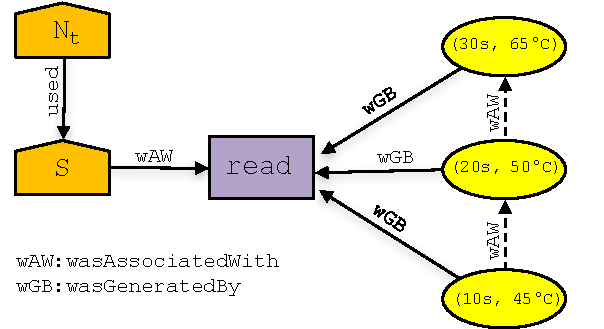
\includegraphics[width=0.6\textwidth]{prov_sensor_v3.pdf}
\end{center}
\caption{Provenance graph generated from a thermostat device.}
\label{prov_sensor}
\end{figure}

\subsubsection{Example: Thermostat}

We demonstrate the Prov-CPS data model with an example of thermostat device ($N_t$) containing a sensor ($S$) that generates temperature readings at a time interval of 10 seconds. Temperature readings of the first 3 consecutive data objects are 45 $\degree$C, 50 $\degree$C, and 65 $\degree$C respectively. Trace events generated for these first three data objects are
\[event_{trace1} = (10 s, 45 ^{\circ}C, read, N_t, S)\]  
\[event_{trace2} = (20 s, 50 ^{\circ}C, read, N_t, S)\]  
\[event_{trace3} = (30 s, 65 ^{\circ}C, read, N_t, S)\]
Relations between components of the trace event are formed as described earlier. $N_t$ forms a \textit{used} edge with $S$, which itself forms a \textit{wasAssociatedWith} edge with the $read$ action. Each temperature reading's timestamp and data object are grouped as a pair ($t, d$) and form a \textit{wasGeneratedBy} edge with the $read$ action and a \textit{wasAssociatedWith} edge with the previous pair associated with $S$ through the $read$ action that generated it. Figure~\ref{prov_sensor} depicts the provenance graph for this thermostat example.



% in which a temperature sensor $s_1$, is connected to device $r_1$. Data object $d$ consists of a set of temperature and humidity values ($i.e., d = \{temperature, humidity\}$). Therefore the tuple representation of trace data for sensor $s_1$ at time $t_1$ is $(t_1, \{temperature, humidity\}, a,  s_1, r_1)$. Since $s_1$ is contained in device $r_1$, $r_1$ forms an edge with $s_1$ with the \textit{actedonbehalfof} relation. (e.g $r_1$ used $s_1$) and $s_1$ forms a \textit{wasGeneratedBy} edge with $a$, activity $a$ forms an \textit{wasusedBy} edge with event $e$. Algorithm \ref{prov_to_trace} further illustrates how a provenance graph can be generated using the provenance-sensor model.





%Sensor data contains observational information such as temperature, and location details which can be transformed to standardized data interchange formats (RDF, XML, JSON). Sensor data are time series data which can be traced over time. Trace data containing sensor readings are important but do not depict dependency relationships when used alone. We transform trace data to provenance to represent causality and dependency relationships between entities in an IoT system. Provenance can be represented as a directed acyclic graph and the edge between two entities is considered a relation. Relations between data objects follows provenance ontology which depicts transformation between entities. We integrate PROV-O and sensor data for better representation of dependency relationships between trace data generated.
%
%\par A single sensor might posses the ability to collect multiple trace data, $td$. For example, a sensor might be able to collect sensor readings of temperature, location, humidity. A combination of trace data at a particular point in time is considered an event. We define an event  for sensor $s_1$ at time $t$ as $e= \{td_1, ...td_n\} $ where $td_1$ is the first trace data collected by $s_1$  and $td_n$ is the last which occurs at time $t$.
%
%\par Adopting provenance ontology to IoT, we represent device information as agents (prov:agents), the operation performed on sensor readings (read, create, update) as a provenance activity (prov:activity), and events as entities (prov:entity). A sensor trace is defined as a tuple  $ (t, e, a, s_1, r_1)$ where $t$ represents a timestamp, $e$ an event, $a$ an operation, $s_1$ sensor information and $r_1$ device information.  

%\begin{algorithm}  
%
%\caption{Provenance-trace Model.}
%\label{prov_to_trace}
%\begin{algorithmic}[1]
%\Procedure{trace2Prov}{$ts$}
%\State \textbf{INPUT: } $ts \gets$ set of trace trace event
%%\State $E_G \gets \{\}$
%%\For{$p_i = (V_i, E_i) \in P, 0 \leq i \leq n$}
%\State $e_{list} \gets \{\}$
%\
%\State $pd \gets pd.createProvDocument()$
%
%\For{  $(t, d, e, c, p \in ts$}
%
%\If{  $c \not\in pd$}
%\State  $ag_c \gets pd.createAgent(c)$
%\EndIf
%
%\If{  $ p \not\in pd$ }
%\State $ag_p \gets pd.createAgent(p)$ 
%\EndIf
%
%\State $dt = \{d, t\}$ 
%
%\State $entity \gets pd.createEntity(dt)$  
%
%\State $e_{list} \gets e_{list} \cup  entity$
%
%\State $activity \gets pd.createActivity(a)$ 
%
%
%\If{$ used \not\in pd$}
% \State  $ pd.used( c, p)$ 
% \EndIf
%
%\State  $pd.wasAssociatedWith(a, c)$
%
% \State $ pd.wasGeneratedBy(a, dt)$ 
% 
% \If{ $counter > 0$}
% \State $ pd.wasAssociatedWith( e_{list}[counter - 1],  entity)$
% \EndIf
% 
%\State $counter = counter + 1$
% 
% \EndFor
%%\EndFor
%\State \textbf{return} $pd$
%\EndProcedure
%
%\end{algorithmic}
%\end{algorithm}

%%%% FIXME: This is wrong. Fix it, or remove it.
%\begin{algorithm}  
%
%\caption{Provenance-trace Model.}
%\label{prov_to_trace}
%\begin{algorithmic}[1]
%\Procedure{Provtrace}{$ts$}
%\State \textbf{INPUT: } $ts \gets$ set of trace trace event
%%\State $E_G \gets \{\}$
%%\For{$p_i = (V_i, E_i) \in P, 0 \leq i \leq n$}
%\State $i = 0$
%\State $e_{list} \gets \{\}$
%\
%\State $pd \gets createProvDocument()$
%
%\For{  $(t, d, a, c, p) \in ts$}
%
%
%\State  $ag_c \gets pd.createAgent(c)$
%\State $ag_p \gets pd.createAgent(p)$ 
%
%\State $entity \gets pd.createEntity(d,t)$  
%\State $e_{list} \gets e_{list} \cup  entity$
%\State $ pd.wasAssociatedWith( e_{list}[i - 1],  e_{list}[i])$ 
%
%\State $activity \gets pd.createActivity(a)$ 
%\State  $ pd.used( ag_c, ag_p)$ 
%\State $pd.wasAssociatedWith(activity, ag_c)$
%\State $ pd.wasGeneratedBy(a, e_{list}[i])$ 
%
%
%\State $i = i+1$
% 
% \EndFor
%%\EndFor
%\State \textbf{return} $pd$
%\EndProcedure
%
%\end{algorithmic}
%\end{algorithm}


\section{Prov-CPS Architecture}
Prov-CPS uses a modular approach that decouples the act of tracing events from that of linking them to form provenance. In this section we describe the architectural design of this approach, and defer implementation details to Section~\ref{system_implementation}.  Figure \ref{framework_design} illustrates the overall system design consisting of four primary components:

%An example of system events are events generated from application source code such as variable, function values or OS system call. Data trace is collected at the tracer component. The resulting output is converted into an appropriate provenance graph representation at the Trace Mapper component using our provenance-trace model as discussed in Section \ref{prov_sensor_model}. The resulting provenance graph generated is stored in a graph database (e.g., Neo4j) for further processing. The generated provenance graph can be used as input to a provenance application of choice. We give a detailed description of components of our framework below:
 
 \textbf{Tracer} is a program located on the CPS device that is responsible for generating trace data from application-level data events. 
  
 \textbf{Trace mapper} converts trace data into a provenance graph representation using the ProvCPS data model in which trace events are mapped to provenance and relationships between them are established.
 
 \textbf{Graph database} is used to store provenance data for further processing. A graph database such as Neo4j is an ideal choice because it allows for easy graph traversal and querying analytics.
 
 \textbf{Provenance application} uses provenance data for specific tasks such as anomaly detection or digital forensics. %For our implementation, we chose to utilize provenance graphs for intrusion detection since we can detect event states changes through causality and dependencies derived from Prov-CPS.
 
 \begin{figure}[h!]
\begin{center}
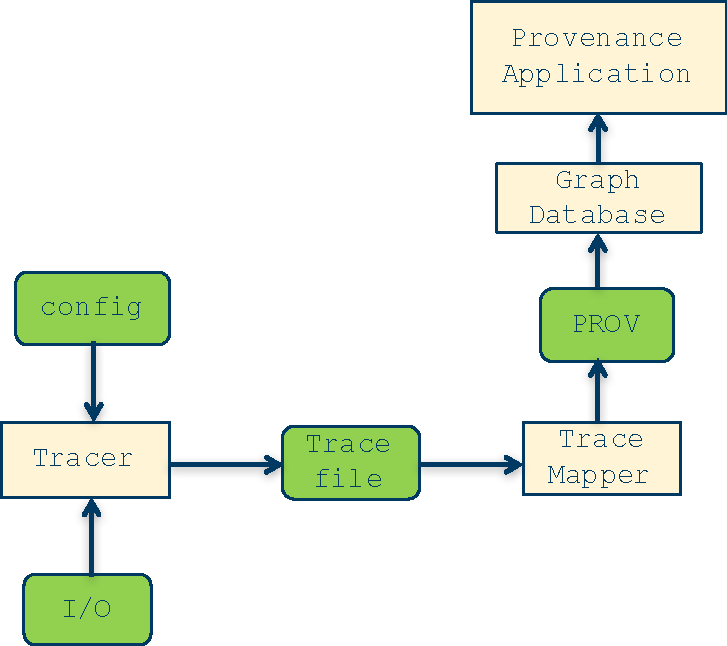
\includegraphics[width=0.6\textwidth]{sys_arc_3_6.pdf}
\end{center}
\caption{Prov-CPS Conceptual System Design.}
\label{framework_design}
\end{figure}

\section{System Implementation} \label{system_implementation}

Figure~\ref{figure} depicts our implementation of the architectural components of Prov-CPS. For the tracer component we use \textbf{barectf}~\cite{barectf}, which is a program for tracing applications written in the C programming language specifically meant for execution on bare-metal devices (devices without an operating system). We chose this program is lightweight, portable, and allows for implementation on memory constrained embedded systems.
%
%since most embedded systems consist of no operating system
%
Barectf generates trace functions that can be called from an application's source code. The event field traced corresponds to values of variables or functions in the application source code that are specified as parameters of the trace function. 
%
%
%Figure~\ref{figure} illustrates source code instrumentation of trace functions in a simplistic temperature and humidity IoT application implemented on a raspberry Pi system.  Trace functions are embedded into the temperature application using functions generated from barectf. Trace function parameter represents event fields of sensor data to be traced. Code fragments highlighted in grey represents trace functions invocation.
%
%%%%Insert source code here... %%%%
%
Event field specification is done by a using a configuration file written in the \textbf{yaml} language from which the trace functions are automatically generated by barectf. At execution time, the trace functions generate trace output to a stream object in \textbf{common trace format} (CTF)~\cite{ctf} packets. CTF is a fast binary trace format for representing trace data.

We implemented a trace mapper on top of the babeltrace~\cite{babeltrace} python bindings for programmatically manipulating CTF streams. With babeltrace, we are able to access trace packets contained in a CTF packet stream and convert them to a provenance graph representation. To generate provenance graphs, we utilize the \textbf{PROV} python library for creating W3C compliant provenance ontology documents. The provenance graph generated is serialized into an intermediate file in JSON format that can be stored in Neo4j for efficient query and graph processing.

The provenance application we use to evaluate Prov-CPS in this work is a graph-based anomaly detection algorithm for use as a CPS intrusion detection system, which we describe in chapter~\ref{sec:prov_anomaly}.

 \begin{figure}[h!]
\begin{center}
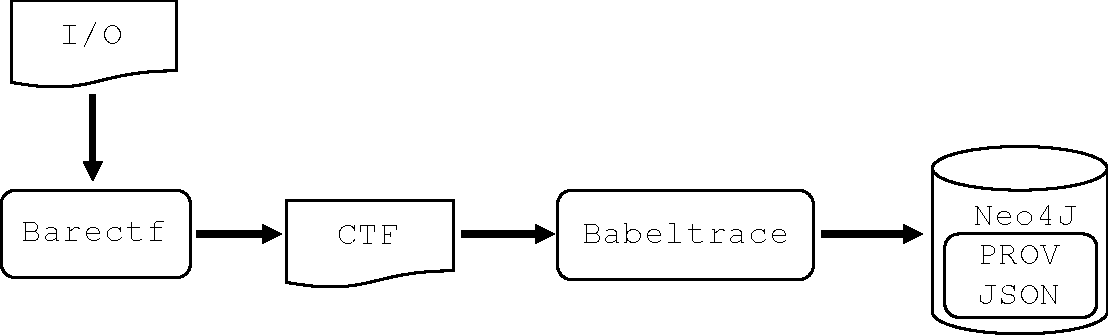
\includegraphics[width=0.6\textwidth]{system_implementation_v4.pdf}
\end{center}
\caption{Prov-CPS System Implementation.}
\label{figure}
\end{figure}

 \subsection{Complexity analysis}
%This section analyzes time and space complexity of the various components contained in Prov-CPS. 

\textbf{Tracer} appends trace data to a list of events. This takes $O(1)$ time and $O(n)$ space. \textbf{Trace mapper} iterates through all of the events and maps them to PROV-O using Provenance-trace model. This takes $O(n)$ time and $O(n)$ space.

\section{Summary}
This chapter introduces PROV-CPS, a provenance collection framework for CPS devices. Components of PROV-CPS such as tracer and trace mapper are discussed with system implementation details. The next chapter discusses storage optimization techniques for provenance data generated in PROV-CPS.







          % Chapter 3
% chap4.tex (Definitions and Theorem)

\chapter{Storage Optimization for Trace Data} \label{MostNarrowEasy}

In this chapter, we explore optimization of provenance graph size using pruning approach. 

%\section{A Policy-Based Approach for Provenance Storage}

\section{Introduction}

%Data provenance captures information flow of across a systems which has applications in forensic analysis, intrusion detection and to scientific research for experiment reproducability. Due to the benefit provenance offers, it has received significant amounts of attention from the scientific community which has led to the development of various provenance-aware applications. For example, PASS \cite{muniswamy_reddy} and HiFi \cite{hi_fi}, both linux based provenance collection system which captures interaction between file level interactions and system calls. Chimera \cite{chimera} and myGrid,  a provenance collection system for scientific workflow reproducibility. These and many more are some of the applications that have been developed as a result of provenance proliferation. In certain cases, provenance generated might be uninteresting to the application. However, one of the major challenge faced by provenance-aware systems is that provenance data incurs additional storage overhead. That is, provenance can easily generate more data than the data in which provenance is is being captured. Our framework, PAIoT is no exception.   The resource constraints imposed on the sensor-actuator and the device layer of the IoT architecture makes storing this data a more challenging task. Table 1 outlines trace and provenance data generated at various event size. We can observe a linear progression in trace and provenance size.  Additionally, due to the large influx of real-time data generated from sensors and actuators, and preliminary results derived, we envision large amounts of provenance data generated from our provenance collection framework.  

%Motivated by the need to provide an optimized storage for provenance data generated, we address the issue of device storage optimization at the trace level by pruning events based on predefined heuristics. Pruning involves the elimination of irrelevant trace data thereby giving way to incoming data. The resultant is a more efficient and sparse representation of the original input trace
%
%The definition of what trace to prune is a challenging task and is often application dependent.



%In this chapter, we make the following contributions:
%
%\begin{itemize}
%
%\item To address the storage issue with automatic provenance collection, we integrate the use data pruning at the trace level to reduce the size of trace data generated. 
%
%\item We develop a data pruning algorithm which produces human readable and semantically meaningful summarized provenance graphs.
%
%
%\end{itemize}

A major challenge faced by any provenance capture system is that provenance data incurs additional storage overhead \cite{issue_provenance}. That is, provenance can easily generate more data itself than data about which provenance is being captured. This storage problem could lead to rapid decline in system performance both in collection and analysis of provenance. Prov-CPS is no exception. Furthermore, the resource constraints imposed on CPS devices further exacerbates the challenge. Table \ref{table:prov_growth} outlines trace and provenance data generated for increasing counts of trace events of a sample application that generates temperature data. 

%We can observe a linear progression in trace and provenance size with respect to time.

%\begin{table}[!b]
%\caption{Trace data size as number of trace increases }
%\label{table:prov_growth}
%\begin{center}
% \begin{tabular}{||c| c| c| c||} 
% \hline
% \textbf{Trace Events} & \textbf{Trace Size (KiB)} & \textbf{Provenance Size (KiB)}  \\ [0.5ex] 
% \hline\hline
% 200 & 8.2 & 25.6 \\ 
% \hline
% 500 & 25.6 & 318.4 \\
% \hline
% 1000 & 51.2 & 642.8 \\
% \hline
% 1500 & 76.8 & 966.5 \\
% \hline
%\end{tabular}
%
%\end{center}
%\end{table}


\begin{table}[!b]
\caption{Trace data size as number of trace increases }
\label{table:prov_growth}
\begin{center}
 \begin{tabular}{||c| c| c| c||} 
 \hline
 \textbf{Trace Events} & \textbf{Trace Size (KiB)} \\ [0.5ex] 
 \hline\hline
 200 & 8.2 \\ 
 \hline
 500 & 25.6 \\
 \hline
 1000 & 51.2 \\
 \hline
 1500 & 76.8 \\
 \hline
\end{tabular}

\end{center}
\end{table}



\subsection{Trace event cost estimation}
To verify the hypothesis that there exists a linear growth in trace and provenance data generated, we provide formulas to estimate the size of provenance and trace events data generated by a device. To calculate the total storage size of trace data generated on a device, we estimate the size of an event. Every event consists of a finite set of event fields such a controller, producer, action. 

%However, information contained in these fields might be encoded as string identifiers with varied sizes. These values can be encoded into a fixed amount of characters and integers. 

The total size of a trace data can be calculated using the function:  \[T_{size} = N_{events} \times K\] where $T_{size}, N_{events}$, represents trace size, and number of events respectively.  $K$ represents the sum of the size of all of the fields contained in an event trace:  \[ K = t_{size} + d_{size}+ a_{size} + c_{size} + p_{size}\] Additionally, given the size of a device, $D_{size}$, the number of trace events that can be stored on a device, $D_{capacity}$, is derived using the function:
%given the number of trace contained in a file
\[ D_{capacity} = \frac{D_{size}}{K} \]


%The total graph size can be calculated by using the formula: \[ G_{size} = \sum{(N_{events} \times (S_{entity} + S_{action}+ X)) + S_{producer} + S_{consumer} } \] where $S_{entity}, S_{producer}$ represents the size of an entity and activity node and $X$ represents the sum of the size of a fixed set of edges per trace event. 


Figure \ref{fig:prov_trace} illustrates the graph of the estimated and actual trace generated from the initial analysis in Table \ref{table:prov_growth}. For calculating the cost of trace events data, the size of each component contained in the trace event is set to 10 bytes. We can observe a linear growth between the estimated and generated data for trace events. 


%\begin{figure*}[!htb]
% 
%\centering
%\subfloat[trace size per events]{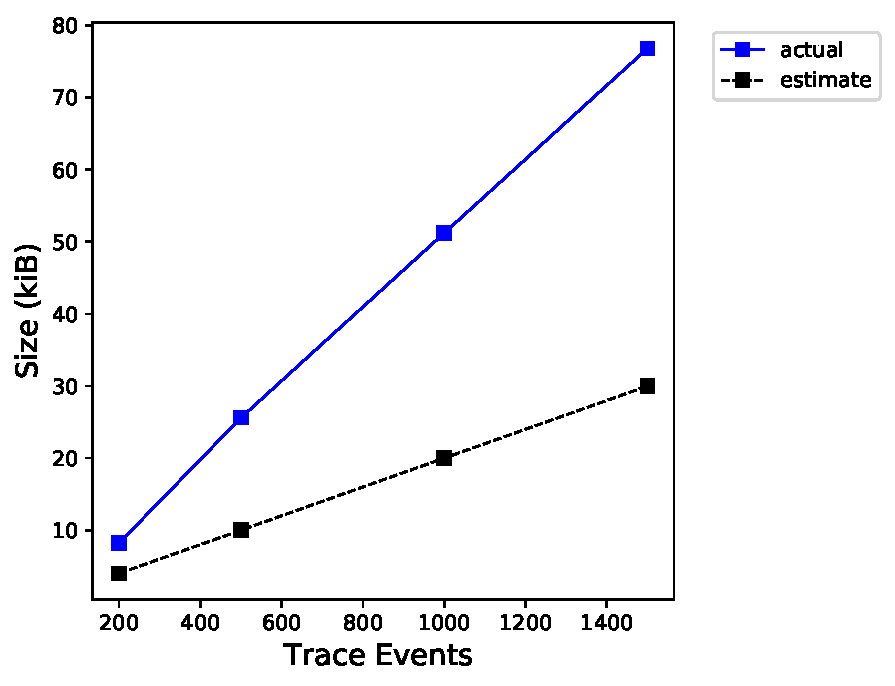
\includegraphics[width=.45\textwidth]{output_trace.pdf}\label{fig:storage_trace}}
%\qquad
%\subfloat[provenance graph size per events]{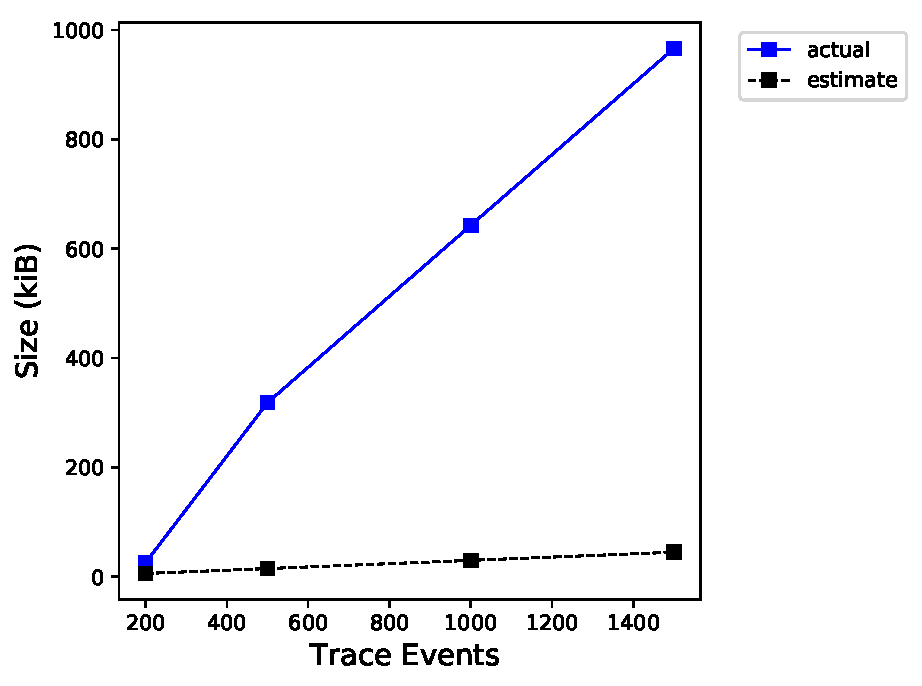
\includegraphics[width=.45\textwidth]{output_prov_1.pdf}\label{fig:storage_prov}}
%%\hfill
%%\subfloat[ROC with Priority Pruning]{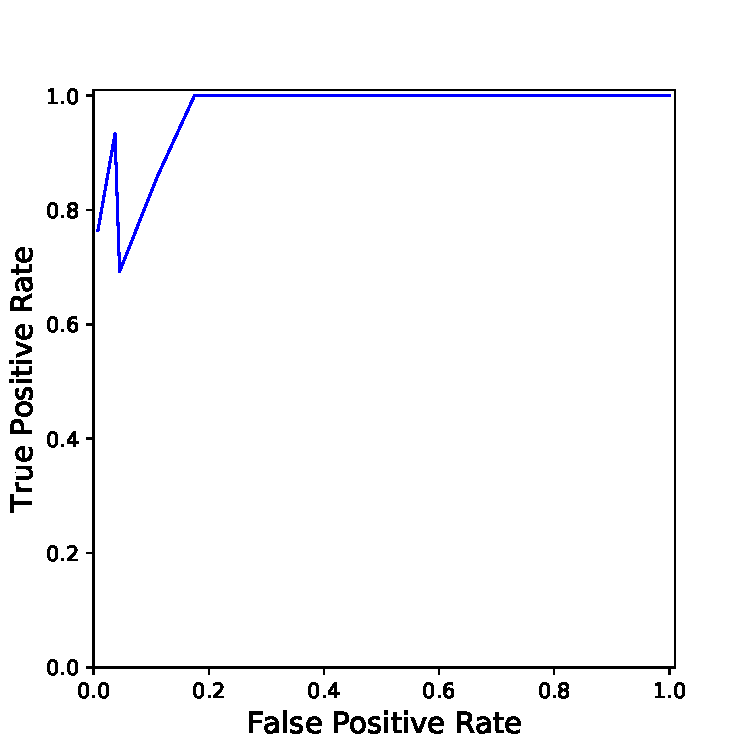
\includegraphics[width=.3\textwidth]{roc_curve_2.pdf}\label{fig:storage_growth}}
%\caption{Storage growth per trace events.}
%\label{fig:prov_trace}
%
%\end{figure*}


\begin{figure}[tbh!]
\begin{center}
%\includegraphics[width=\textwidth]{vector3.pdf}
%\includegraphics[width=\textwidth]{vector5.pdf}
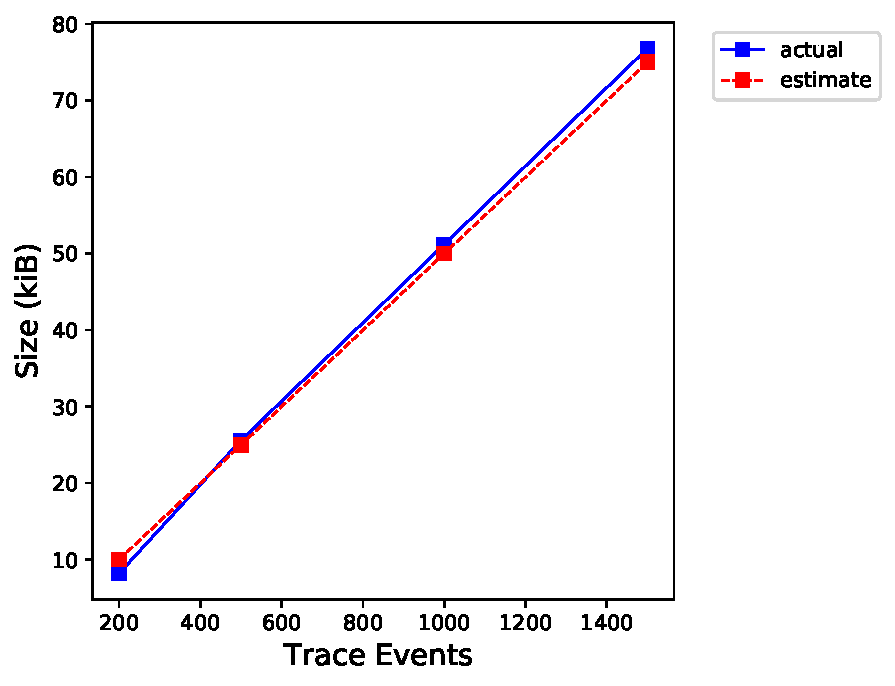
\includegraphics[width=.6\textwidth]{output_prov_trace.pdf}
\end{center}
\caption{Storage growth per trace events. }
\label{fig:prov_trace}
\end{figure}



%It is important to note that the estimated provenance graph is an approximate scalar multiple of the actual graph size which is due to the additional storage overhead from provenance graphs serialization to JSON. 

%The Algorithm defines a fixed set of edges per trace events and each event creates a new node. 


Motivated by the need to provide an optimized storage for provenance data generated, we address the issue of device storage at the trace level by pruning events based on predefined heuristics. Pruning is defined as eliminating unwanted events in a trace to optimize storage space. %We develop a data pruning algorithm which produces human readable and semantically meaningful provenance trace. The resultant is a more efficient and sparse representation of the original input trace. More information on the pruning heuristic used is discussed in section \ref{Pruning}. 


 

\section{Types of Provenance Pruning} 
To determine what data to prune is a challenging task and often application dependent.  %For example, provenance data might be considered uninteresting until it has been modified by a malicious instance. 
%braun2006issues
Based on the current state of the art, the common approaches to data pruning are:
 
\textbf{Pruning at collection} removes provenance during or before the collector stores it. For example, an application might decide to eliminate repeated trace data as they are generated, or a system-call provenance collector in an operating system kernel might ignore user configuration and temporary files that are unnecessary for the provenance application use case.

\textbf{Pruning after collection}  involves removing unwanted provenance information after provenance has been saved to a storage system. %For example, we can target attributes that are found in every trace event.

\textbf{Policy-based pruning} \cite{Bates:2015:TOY:2814579.2814586} involves the use of user-specified conditions (expressed as a policy) to determine data to prune. Policy offers a flexible method of pruning, but requires a robust policy language to express policy decisions, which often could be a challenge to design. A policy is evaluated by a decision point  that returns accept or deny. %So far, to the best of our knowledge,~\cite{bates_towards_2013} is the only policy-based approach described in the literature.

%\textbf{Graph Summarization} \cite{compressing_graph, Tian, Navlakha} involves aggregating graph nodes and edge relationships based on similar attributes without loosing information contained in the original graph. This reduces the size of the original graph while preserving the structural pattern of node and edge relationships.  

\textbf{Compression}~\cite{xie11-tapp,hussain_secure_2014, 7038199} involves reducing the size required to represent a data value. Provenance compression may be applied to the provenance or to its graph structure. The use of lossy or lossless techniques can be employed in provenance pruning, but the existing literature advocates for lossless approaches.

\textbf{Graph summarization} involves aggregating graph nodes and edge relationships based on similar attributes without loosing information contained in the original graph. This reduces the size of the original graph while preserving the structural pattern of node and edge relationships. The structural pattern of provenance graph consists of homogeneous nodes (i.e., entity, agent, activity) which can be harnessed to provide attribute-based summarization to an original graph structure. Summarization improves graph visualization and allows for better understanding of graph structures and relationship between various node and edge interactions.

\section{Pruning in Prov-CPS} \label{Pruning}
Our approach involves pruning at collection by selectively dropping events from the set of captured traces. We introduce two techniques for provenance pruning: first-in, first-out (FIFO) and prioritized.  
\begin{enumerate}

%\item\textbf{Least-$k$ queue-based pruning:}  

\item\textbf{FIFO pruning:}  
  FIFO is the na\"ive approach that uses the natural order of arrival time to select events to discard. As trace events are generated they are added to a FIFO. Once the queue has reached its capacity, each new trace event causes the oldest trace event in the FIFO to be eliminated. An advantage of FIFO pruning is that it can be implemented without application knowledge. A disadvantage is that it is not selective in what it discards, and if provenance becomes more important (for a given provenance application) as it becomes older, then FIFO is not a good choice.
%  Each event traced is stored in a queue, $Q$ where $Q= \{ q_1,...,q_n\}$. We define the queue capacity, $c$ as the maximum size of the queue. When the size of $Q$ exceeds $c$, the last $k$ element is truncated from $Q$ and the incoming trace data is appended to the end of $Q$. $k$ can be defined by application logic or by the user.

\item \textbf{Prioritized pruning:}
The prioritized approach assigns a priority value to each event as it is traced based on an application defined priority, thus it extends the definition of the trace event with an additional field for the priority value. Although application knowledge is required to determine the priority of each event, many CPS application domains include natural priority values that can be immediately leveraged by the provenance application. With this approach, lower priority events are discarded from the set of trace events first. A drawback of this approach is the cost needed to sort trace events when there are many priority values.

% This technique is similar to the na\"ive approach however, the key difference is the use of application defined logic contained in each trace event as a means to assign priority value.
% For example, in a CAN protocol bus~\cite{can_bus}--a popular messaging protocol used by in-vehicular devices (Electronic Control Units) to communicate with each other, two messages transmitted on a can bus at the same time undergo an arbitration process which involves choosing what messages are first transmitted on the network bus. Priority is given to an ECU with low id. That is, an id with a lower number always wins the arbitration process. This idea can be leveraged to perform pruning where messages with higher message ids are placed at the end of the queue. Once the queue reaches its capacity, $k$ messages are truncated to give room for new messages which are appended at the end of the queue.
\end{enumerate}

\subsection{Complexity analysis}
\textbf{FIFO Pruning} is implemented using a queue data structure. This takes constant time $O(1)$ to insert and delete events from queue. Since there are $n$ elements contained in the queue, the worst case space utilized is $O(n)$. \textbf{Priority-based pruning} is implemented using a heap data structure. It takes $O(\log{}n)$ to insert and delete elements contained in the heap with a space complexity of $O(n)$.

\section{Summary}
This chapter motivates the need for storage optimization in PROV-CPS. Two pruning heuristics, FIFO and Priority-based pruning, were proposed to address the issue of the storage overhead generated by PROV-CPS. The next chapter introduces a provenance-based anomaly detection system for the detection of anomalous instances through information flow of device events. 

%Graph summarization is a process of aggregating graph nodes and edge relationships based on similar attributes without loosing information contained in the original graph. This reduces the size of the original graph while preserving the structural pattern of node and edge relationships. The structural pattern of provenance graph consists of homogeneous nodes (i.e., entity, agent, activity) which can be harnessed to provide attribute-based summarization to an original graph structure. Summarization improves graph visualization is allows for better understanding of graph structures and relationship between various node and edge interactions. One major challenge with summarization is dealing with the complexity and volume of data generated and also with complex dependency relationships that exists between nodes.
%
%
%Graph summarization also has applications in clustering, classification, outlier detection \cite{Smets2011TheOO}, graph query optimization and understanding the interaction of large graph dataset through visualization.
%
%For this dissertation, we are focused on using graph summarization of provenance graphs for storage optimization.
%
%
%% Summarization allows users to make sense of data through visualization and also as a storage optimization technique.
%
%
%
%In this chapter, we make the following contributions:
%
%\begin{itemize}
%
%\item To address the storage issue with automatic provenance collection, we integrate the use of graph summarization by grouping specific node/edge relationship to reduce the original graph size. 
%
%\item We develop a graph summarization method which produces human readable and semantically meaningful summarized provenance graphs.
%
%\item We evaluate our provenance summarization algorithm on a dataset from an automotive domain. Our experiment calculates the percentage of storage savings(i.e., size difference) by comparing the size of the resulting summarized provenance graph to the original graph.
%\end{itemize}
%
% The remaining part of this chapter are outlined as follows. Section 2 discusses types of graph summarization, section 3 talks about our rational for graph summarization. 
%
%  
% 
% \subsection{Graph Summarization Characteristics}
%
%Due to the intricate dependency relationship that might exist between node contained in a provenance graphs and also based on the application use case, most provenance graphs are input to some real time computation on the provenance graphs, a provenance graph summary should satisfy the following characteristics:
%
%\begin{itemize}
%\item \textbf{Completeness.} A summarized graph should reproduce provenance data as contained in the original graph in a manner that preserves information contained in the node and edges of the original graph without loosing information contained. 
%
%\item \textbf{Efficiency.} Since provenance data typically consists of massive dataset of graph data, a provenance summary should produce a concise representation of the original graph which helps speed up graph processing.  
%
%\item \textbf{Queryable.}  A summarized provenance graph should represent a compact representation of the original graph which can be efficiently queried without loss of information.  
%
%\end{itemize}
%
%We satisfy the requirements listed above by aggregating the contents of similar nodes contained in the provenance graph based on defined attributes. More information on our approach is discussed in section \ref{}
%
%
%
%\subsection{Graph Summarization Techniques}
% 
%% Types of graph summarization are outlined below as follows: 
%
%There has been a considerable amount of prior work done on graph summarization \cite{grass, compressing_graph, Tian, Navlakha, hussain_secure_2014} most of which are application specific. Some of the prior work focuses on storage space reduction \cite{grass, Tian, Navlakha} using attributes while others focuses on bit compression \cite{compressing_graph, hussain_secure_2014} and  techniques. Below are the types of summarization technique used based on prior work.
%
%\begin{itemize}
%
%\item \textbf{Grouping or aggregation based approach.} This is one of the most popular approach in which nodes and edges with similar attributes are aggregated. Grouping based approach is classified into two categories:
%
%\begin{itemize}
%
%\item \textit{Node grouping} involves two types: Clustering approach in which node in densly located node clusters are grouped into a single node referred to as a super-node. The other approach involves grouping nodes with similar attributes into a super-node based on a defined attribute or structure. 
%
%\item \textit{Edge grouping} involves aggregating edges with similar attributes into compressor or virtual nodes. Compression in this case refers to replacing a set of edges into a node. 
%
%\end{itemize}
%
%\item \textbf{Compression-based approach} employs the use of compression algorithms (lossy and lossless approach) to reduce the number of bits required for each node and edge contained in the provenance graph.
%
%\item \textbf{Simplication or prunning approach} eliminates unimportant nodes or edge relationship contained in a graph. The challenge is in determining what is considered unimportant which is often times application specific. The resultant summarized graph produced is a sparse representation of the original graph.
%
%\item \textbf{Statistical-based approach.} employs the use of statistical methods such degree distribution, hop-plot, and clustering co-efficient for edges and node aggregation.
%
%\end{itemize}
%
%\section{Comparing graph summarization to other storage optimization approach}
%
%\begin{itemize}
%
%\item \textbf{\textit{Policy-based prunning}}: There has been a limited amount of prior work on policy-based pruning for provenance. Bates et al \cite{Bates:2015:TOY:2814579.2814586}. proposed a policy based approach which enforces ppruning at the OS based on MAC policies. Summarization helps reduce storage cost while discovering structural patterns that exists in the original input graph. With policy-based pruning, lossy optimization techniques is often utilized as a means of elimimating unimportant information contained in the provenance graph. The definition of data considered unimportant is relative and domain specific. One might argue that pruning provenance data removes provenance data originality. (i.e., the lineage of data has been tampered with) since it deletes from the history. 
%
%
%\item \textbf{\textit{Compression}}: Although summarization and compression might seem related since they both involve combining nodes and edges with a resulting space optimized graph, they are quite different. Compression focuses on minimizing graph edges without the need to produce a summarized graph. For example, a compression techniques can be applied to a whole graph without preserving graph structure. Graph summarization on the other hand leverages compression to generate an efficient graph summary from an input graph while maintaining structural patterns that might exist in the original graph.
%
%\end{itemize}
%
%
%\par Both policy-based prunning and compression are complementary to graph summarization. That is, both are more effective when used in combination with graph summarization techniques. To this effect, our approach utilizes a combination of node aggregation, bit compression and pruning techniques to ensure optimal space savings.
%
%
%\section{Our Approach}
%
%Provenance graph contains redundant information such as edge and node labels. Also, we group nodes based on activity type with time dependency. That is nodes that occur successively with the same activity are grouped as one super-node. Also, we introduce the use of the pruning approach whereby we remove nodes based on user specified attributes.Our algorithm makes use of bit compression, graph aggregation and prunning approach to optimize space savings.
%
%
%
%
%
%\section{Related Work}
%
%
%\section{Experimental Evaluation}

%
%Since organizations have varied provenance requirement(s), making a static provenance policy is not suitable for the IoT. Using policy for storage optimization is slightly different from the typical use of policy in enforcing access control.  For the IoT framework, the product manufacturer is considered a policy creator. This reduces the complexity of creating and managing policy documents by the IoT device consumers. A policy creator is a user which has the right to add, delete or modify a policy document. A policy document is required to specify which provenance data to collect thereby providing storage access to provenance unlike system access control which evaluates user access rights to view a resource. 
%
%
%
%
%
%\par 
%
%The policy framework consists of a policy engine. The policy engine contains authorization and enforcement components that provides and enforce decisions on how provenance data should be stored. A policy document is a component of the policy framework. It identifies provenance data that is considered relevant to the IoT application. Our policy architecture is modeled using the Common Open Policy Service (COPS) Standard \cite{rfc2748}. COPS consists of components for policy generation, evaluation and enforcement. The Policy Enforcement Point (PEP) enforces decisions received from the Policy Decision Point (PDP). The PDP evaluates policies and generates decision based on the evaluation. The model can be extended to include a secondary decision point (SDP) which allows for distributed policy evaluation, thus freeing up the PDP from communication bottlenecks caused by large amounts of requests received by a single PDP. Figure \ref{policy_architecture} below illustrates the system architecture of our proposed policy-based storage framework. Different layers of the IoT architecture contain different decision and enforcement components. The sensor-actuator layer of the IoT architecture is omitted because it has negligible memory resources and the  sensors and actuators are usually physically part of a device in the device layer and as such does not have any data to prune. 
%
%
%Policy document which is generated by the policy creator serves as an input to the PDP component and is evaluated at the device, gateway and cloud layer. The PEP which is involved with generating requests is located in the device and gateway layer. SDPs can be located in the gateway layer, which allows for policy evaluation without incurring additional network overhead of communicating with the PDP located in the cloud layer. 


         % Chapter 4
% chap5.tex (Definitions, Theorem and Proof)

%\chapter{CPS Device Sensor Data Anomaly Detection using Provenance Graphs}
%\chapter{Anomaly Detection using Provenance Graphs}
\chapter{Provenance-Based Anomaly Detection} \label{sec:prov_anomaly}
This chapter discusses the application of provenance data for intrusion detection of malicious events in a CPS device. We propose an approach to identifying anomalous sensor events using provenance graphs. This approach involves the use of a similarity metric to compare observed provenance graphs with provenance graphs derived from an application's normal execution. The result is an anomaly score which is  compared with a previously set threshold to classify an observed provenance graph as either anomalous or benign. We evaluate the effectiveness of our approach with a sample IoT application that simulates a climate control system.
 
 \par Our method of comparing the similarity of provenance graphs was inspired by an information retrieval technique for document retrieval. Given a corpus $D = \{ d_1,..., d_n\}$, and query, $q$, how do we find document(s) $\{d_x,....d_y\}$ which are similar to $q$ and rank them by order of importance. To achieve this, documents contained in the corpus are converted into a vector space representation which allows documents to be ranked based on some similarity metric.


\section{Graph Similarity} \label{similarity}
Similarity is a measure of how identical two objects are, for example, by measuring the angle between objects (using cosine similarity) or a linear distance (using euclidean distance) between the objects. In this work, we use cosine similarity as our similarity metric. Cosine similarity is a measure of orientation between two non-zero vectors. It measures the cosine of the angle between the vectors. Two vectors which are at an angle of 90$\degree$ have a similarity of 0, two vectors which are identical (with an angle of 0\degree) have a cosine of 1, and two vectors which are completely opposite (with an angle of 180\degree) have a similarity of -1. Since we are concerned with the similarity between vectors, we are only concerned with the positive values bounded in [0,1]. The cosine similarity between two vectors, $X$ and $Y$, is computed by:

\[\mathbf{\cos{(\theta)}} = \dfrac{X \cdot  Y}{ \lVert \mathbf{X} \rVert \cdot \lVert \mathbf{Y} \rVert} =\dfrac{\sum_{i}^n X_i Y_i }{\sqrt[]{\sum_{i}^n X_i^2} \times \sqrt[]{\sum_{i}^n Y_i^2}}  \]

%Algorithm \ref{alg:graph_similarity} describes how to calculate the cosine similarity of two graphs $p_x, p_y$ given their vector representations $u_x, u_y$

%Each graph consist of an edge list which contains all edges contained in the provenance graph.

\par In order to apply cosine similarity between provenance graphs, we compute a vector representation which reduces the graph into an $n$-dimensional vector space where $n$ represents the total number of edges contained in the union of all edge sets. Figure \ref{prov_vector} illustrates the vector space conversion of provenance graphs. $\boldsymbol{G_1}$, and $\boldsymbol{G_2}$ which consists of vertices $A,B,E,F,G, I, J, L, S, R$ and edge labels $used, wAW, wGB, wDB$. The vector space representation of $u_1$ is the occurrence of edges contained in the edge set of graph $G_1$, which  are also found in the collective union of edge sets. Algorithm \ref{graph_to_vector} further outlines the concept of graph to vector conversion.

\begin{figure}[h!]
\begin{center}
%\includegraphics[width=\textwidth]{vector3.pdf}
%\includegraphics[width=\textwidth]{vector5.pdf}
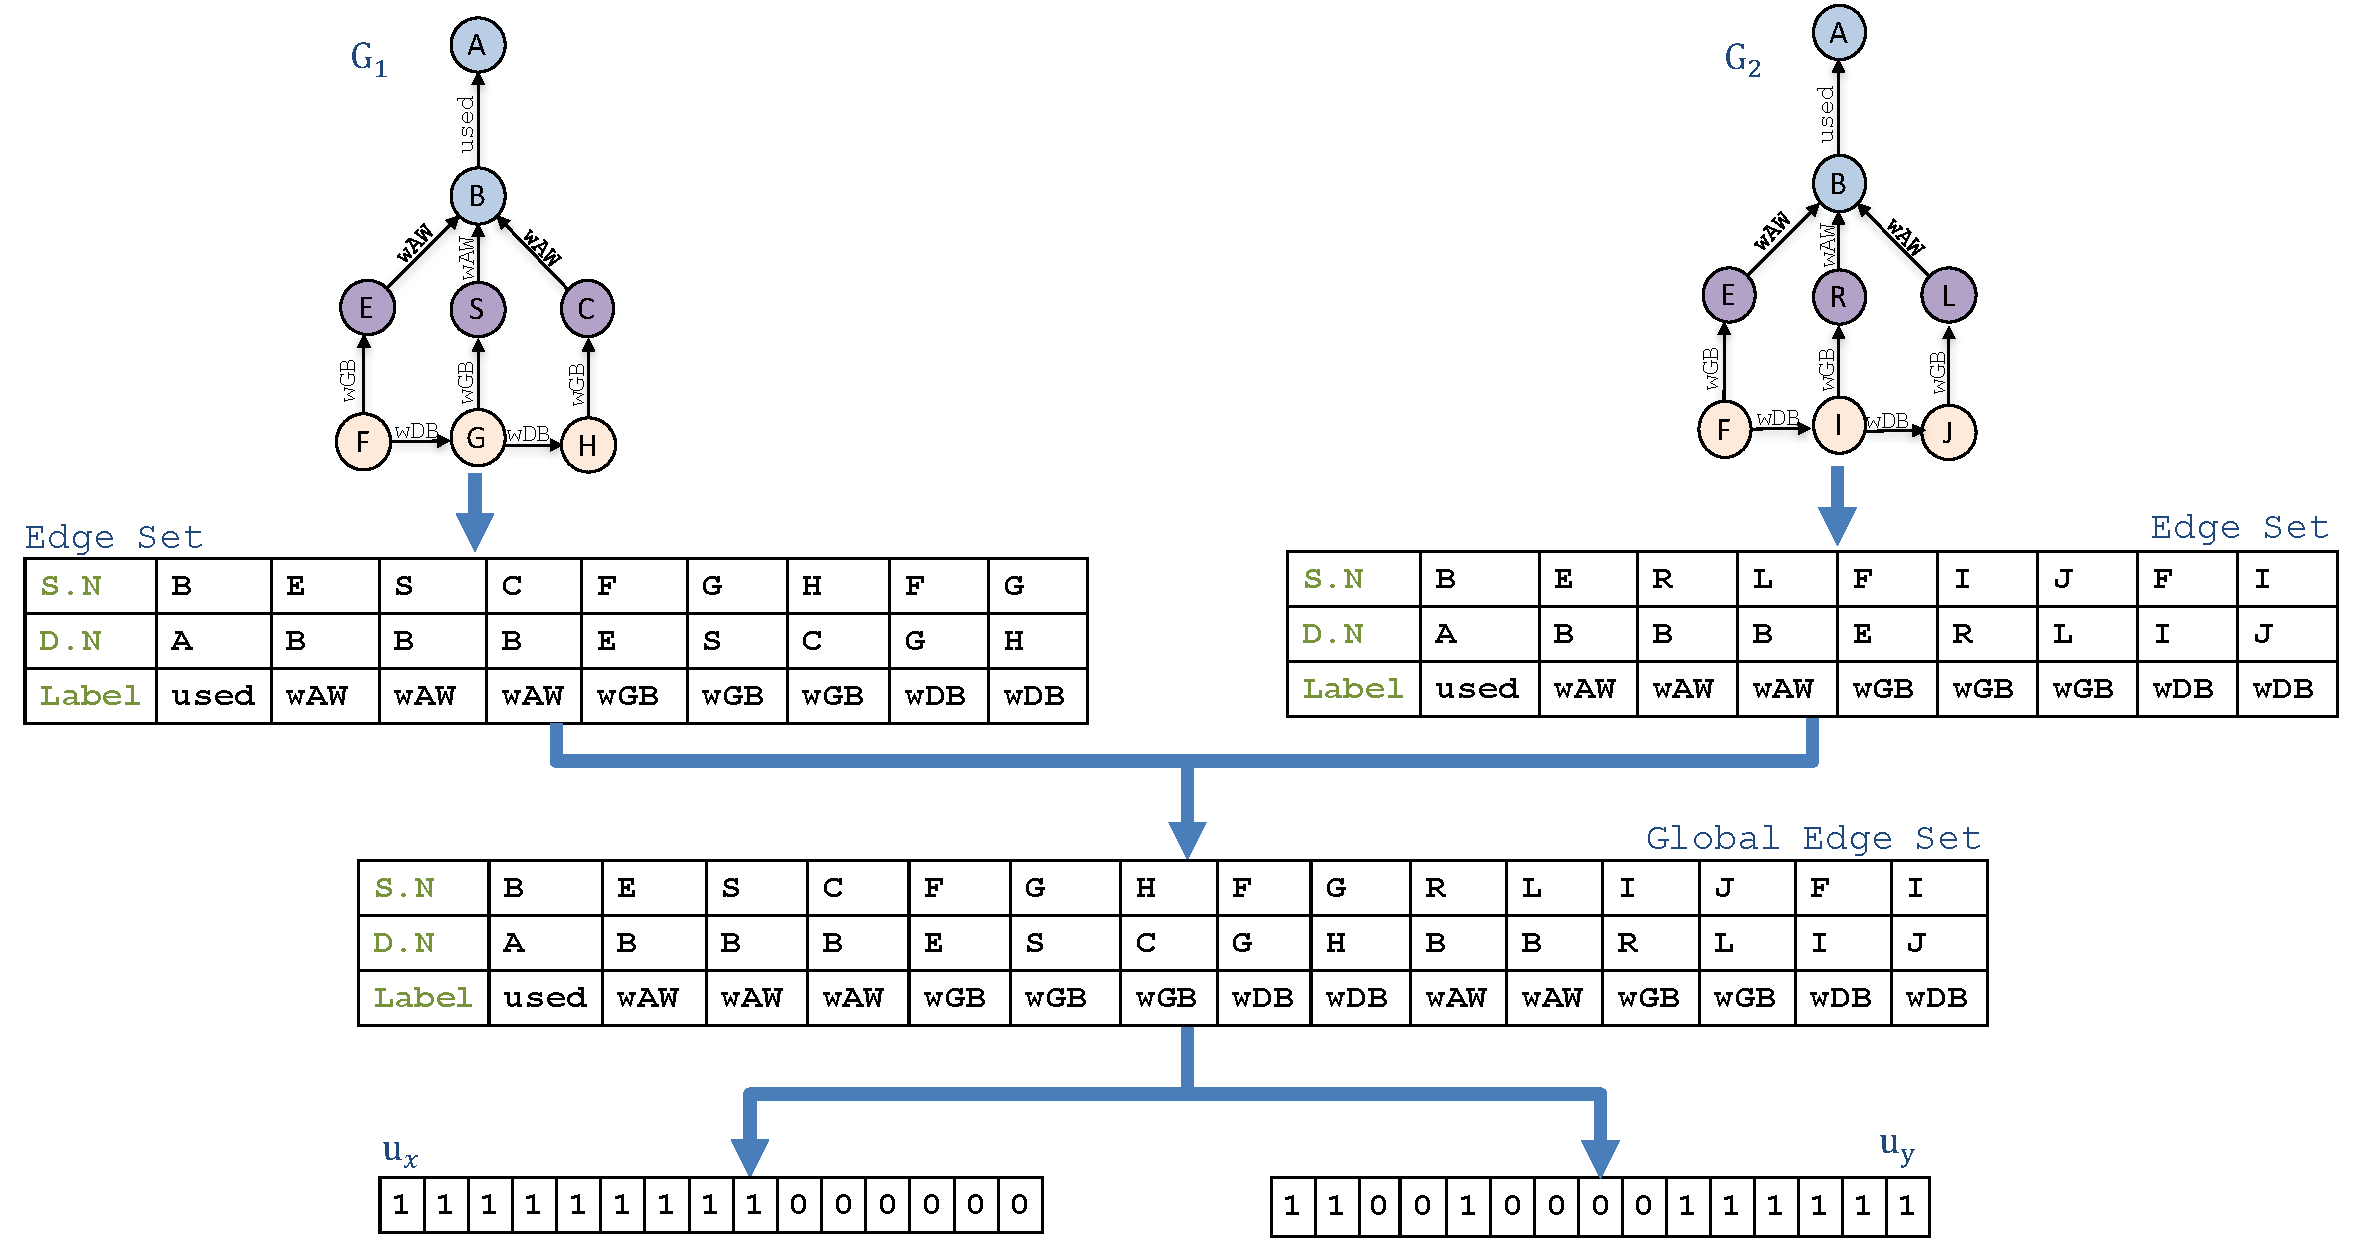
\includegraphics[width=\textwidth]{Picture_13_edit_5.pdf}
\end{center}
\caption{Provenance graph conversion to vector space. $u_x, u_y$ represents vectors generated from both provenance graphs and labels are an abstraction of $(type, value)$ tuple. }
\label{prov_vector}
\end{figure}

\section{Anomaly Detection on Provenance Graphs}
Anomaly detection involves the use of rule-based, statistical, clustering or classification techniques to determine normal or anomalous data instances. The process of determining all anomalous instances in a given dataset is a complex task. A major challenge in anomaly detection is providing the right feature set from the data to use for detection. Another challenge exists in defining what constitutes as normal system behavior. Most anomaly detection using point-based data often fail to include the dependencies that exist between data points. 

\par Due to the ubiquitous nature of CPS devices, there are a wide array of vulnerabilities associated with them. In designing our anomaly detection framework, we expect an attacker's footprint is reflected through the data flow as depicted in the provenance graph. Our algorithm detects attacks such as false data injection, and state change as depicted in information flow of sensor events in provenance graphs.

\begin{algorithm}[h!]  
\caption{Graph to vector conversion.} 
 \label{graph_to_vector} 
\begin{algorithmic}[1]

\Procedure{GraphtoVector}{$E, E_G$}

\State $n \gets |E_G|$

\State $Q[k],Q[i] \gets 0, 0 \leq i < n$

\For{$e_j \in E$}

%\State \textit{Found} $\gets$ \textbf{False}

\For{$e_g \in E_G \mid 0 \leq g < n$}

%\If{$e_j \sim e_g$}
\If{$e_j = e_g$}
\State $Q[g] \gets Q[g] + 1$
%\State \textit{Found} $\gets$ \textbf{True}
\EndIf

\EndFor

\EndFor


\State \textbf{return} $Q$

\EndProcedure

\end{algorithmic}
\end{algorithm}


\begin{algorithm}[h!]

\caption{Detection algorithm given an observation phase graph set, $P$, a detection phase graph, $G$, and a threshold $T$.} 
 \label{alg:graph_anomaly} 

\begin{algorithmic}[1]  

\Procedure{GraphAnomaly}{$P,G,T$}

\State \textbf{INPUT: } $P=\{G_0,...,G_n\} \mid G_i\gets (V_i, E_i), 0 \leq i \leq n.$

%\State $E_G \gets \{\}$
%\For{$p_i = (V_i, E_i) \in P, 0 \leq i \leq n$}
\State $E_G \gets \cup_{i=0}^{n} E_i$

\State $Q \gets GraphtoVector(G, E_G)$ 

\State $Z \gets \{\}$

\For{$G_i \in P$}
\State $N_i \gets GraphtoVector(G_i, E_G)$

\State $z \gets Cosine\_Similarity(Q, N_i)$

\State $Z \gets Z \cup z_i$

\EndFor	

\State $s_{val} \gets max(Z)$

\If{ $s_{val} \geq T$}
\State \textbf{return} normal

\EndIf

\State \textbf{return} anomaly
\EndProcedure
\end{algorithmic}
\end{algorithm}

\par Many CPS devices implement a control systems in which sensor data is used as an input in a feedback loop to an actuator. The operations of most control systems are regular and predictable. For example, in a thermostat application, temperature readings generated might be converted from Celsius to Fahrenheit and utilized as feedback to an actuator. Each iteration of a control loop sequence generates a path in a provenance graph. This notion can be leveraged to define an expected provenance graph for each application. 

\par The expected regularity of provenance graphs in CPS applications motivates a supervised learning approach to anomaly detection. This approach consists of two phases: observation phase, also known as the training phase, and the detection or test phase. In the observation phase, the system collects provenance data considered to be a representation of the normal system behavior. In the detection phase, the provenance graph set is compared with the provenance graph derived from subsequent observations to determine if an anomaly exists by measuring similarity between this graph and the provenance graph set. Note that provenance graphs from the observation and detection phase form a graph set. A global edge set, $E_G$ represents the union of edge sets contained in a graph set. Algorithm \ref{alg:graph_anomaly} is the graph anomaly detection function given an observation phase graph set, $P$, and a detection phase graph, $G$. $Z$ represents a list of the cosine scores from comparing each of the provenance graphs in the observation phase graph set with a detection phase graph. The maximum cosine similarity score of elements contained in $Z$ is taken as the score for the detection phase graph, and if that score is above the threshold $T$ then the graph is considered normal, otherwise it is classifed an anomaly.

\subsection{Defining Anomaly Threshold}

An anomaly threshold $T$ is a score that defines at what point a provenance graph contained in the test data is considered anomalous. Ensuring a proper threshold score is used for detection is an important task that requires extensive knowledge of the application domain. The threshold often is manually set to a value that is defined by domain experts. For automatic anomaly threshold detection, one can use prediction methods to define an anomaly score. Threshold values can be increased or decreased to alter the anomaly detection accuracy.




%\begin{algorithm}
%\caption{Cosine similarity given two vectors.}
% \label{alg:graph_similarity}
% 
%\begin{algorithmic}[1]
%
%\Procedure{sim}{$u_x,u_y$}
%\State \textbf{INPUT: } $u_x=\{u_{x_0},...,u_{x_n}\},u_y=\{u_{y_0},...,u_{y_n}\}$
%\State $S_p, S_{u_x}, S_{u_y} \gets$ 0
%%\State $S_{ux} \gets$ 0
%%\State $S_{uy} \gets$ 0
%\For{$ 0 \leq i \leq n$}
%
%\State $S_p \gets S_p + (u_x[i] \times u_y[i])$
%\State $ S_{u_x} \gets  S_{u_x} + u_x[i]^2$
%\State $S_{u_y} \gets S_{u_y} + u_y[i]^2$
%
%\EndFor
%
%\State $G \gets \dfrac{S_p}{\sqrt[]{S_{u_x}} \times \sqrt[]{S_{u_y}} }$
%
%%\State $G \gets S_p \div \sqrt[]{S_{ux} \times S_{uy}}$
%
%\State \textbf{return} $G$
%
%\EndProcedure
%
%\end{algorithmic}
%
%\end{algorithm}
%
%\begin{algorithm}
%\caption{Algorithm to construct the global edge set}
%
%\begin{algorithmic}[1]  
%\caption{Construction of global edge set from a set of provenance graphs.}
%\label{graph_to_globaledgelist}
%
%\Procedure{GraphSetToGlobalEdgeSet}{$P$}
%\State \textbf{INPUT: } $P=\{p_0,...,p_n\} \mid p_i\gets (V_i, E_i), 0 \leq i \leq n.$
%
%%\State $E_G \gets \{\}$
%%\For{$p_i = (V_i, E_i) \in P, 0 \leq i \leq n$}
%\State $E_G \gets \cup_{i=0}^{n} E_i$
%
%%\EndFor
%\State \textbf{return} $E_G$
%
%\EndProcedure
%
%\end{algorithmic}
%\end{algorithm}
%
%
%\begin{algorithm}[h!]  
%\caption{Graph to vector conversion.} 
% \label{graph_to_vector} 
%\begin{algorithmic}[1]
%
%\Procedure{GraphtoVector}{$E, E_G$}
%
%\State $n \gets |E_G|$
%
%\State $Q[k],Q[i] \gets 0, 0 \leq i < n$
%
%\For{$e_j \in E$}
%
%%\State \textit{Found} $\gets$ \textbf{False}
%
%\For{$e_g \in E_G \mid 0 \leq g < n$}
%
%%\If{$e_j \sim e_g$}
%\If{$e_j = e_g$}
%\State $Q[g] \gets Q[g] + 1$
%%\State \textit{Found} $\gets$ \textbf{True}
%\EndIf
%
%\EndFor
%
%\EndFor
%
%
%\State \textbf{return} $Q$
%
%\EndProcedure
%
%\end{algorithmic}
%\end{algorithm}
%
%\begin{algorithm}[h!] 
%\caption{Calculates an anomaly score given a set of cosine similarity values.}  
% \label{alg:min_func} 
%\begin{algorithmic}[1]  
%
%\Procedure{calculateAnomalyScore}{$Z$}
%\State \textbf{INPUT: } $Z=\{z_0,...,z_n\} , 0 \leq i \leq n.$
%\State score $\gets 0.0$
%\For{$z_i \in Z$}
%\If{score $> z_i$}
%\State score $\gets z_i$
%\EndIf
%\EndFor	
%\State \textbf{return} score
%\EndProcedure
%
%\end{algorithmic}
%\end{algorithm}
%
%
%\begin{algorithm}[h!]
%
%\caption{Detection algorithm given an observation phase graph set, $P$, a detection phase graph, $p$, and a $threshold$.} 
% \label{alg:graph_anomaly} 
%
%\begin{algorithmic}[1]  
%
%\Procedure{GraphAnomaly}{$P,p,threshold$}
%
%\State $E_G \gets GraphSetToGlobalEdgeSet(P \cup p)$
%
%\State $Q \gets GraphtoVector(p, E_G)$ 
%
%\State $Z \gets \{\}$
%
%\For{$p_i \in P$}
%\State $N_i \gets GraphtoVector(p_i, E_G)$
%
%\State $z \gets SIM(Q, N_i)$
%
%\State $Z \gets Z \cup z_i$
%
%\EndFor	
%
%\State $s_{val} \gets calculateAnomalyScore(Z)$
%
%\If{ $s_{val} \geq$ threshold}
%\State \textbf{return} normal
%
%\EndIf
%
%\State \textbf{return} anomaly
%\EndProcedure
%
%
%
%\end{algorithmic}
%
%
%
%\end{algorithm}



%\section{Summary and Conclusion}
%
%In this paper, we propose an anomaly detection algorithm for detecting anomalous instances of sensor based events in an IoT device using provenance graphs. We evaluate our approach with a preliminary study on an IoT application which simulates a climate control system. In the future, we plan on conducting further experimentation to identify the false and true positive rates of our algorithm using select IoT application dataset. 




%\section{Acknowledgment}
%This research has been supported in part by US National Science Foundation (CNS grant No. 1646317). Any opinions, findings and conclusions or recommendations expressed in this material are those of the author(s) and do not necessarily reflect the views of NSF.




         % Chapter 5
% chap6.tex (Significance and Future Work)

\chapter{Experiments}

In this chapter, we evaluate Prov-CPS using our anomaly detection algorithm on a climate control system and an automotive network bus.

\section{Climate Control System}
The experiment evaluation serves as a preliminary study to confirm the correctness of our theoretical approach in detecting anomalous instances between provenance graphs. We evaluate our intrusion detection algorithm on Prov-CPS by implementing an application which simulates a climate control system. Climate control systems ensure a proper functional environment for people and machinery. Constant irregularities in temperature could have devastating effects on industrial machinery. This system consists primarily of a heating ventilation and air conditioning (HVAC) system which uses temperature and humidity data to regulate environmental conditions within a building. We utilize a publicly available dataset \cite{LANGEVIN201594} which consists of a year's worth of longitudinal data on the thermal conditions, related behaviors, and comfort of twenty-four occupants in a medium-sized building generated at  a period of fifteen minutes. We utilize the temperature and humidity data as input to our simulation. We generate provenance graphs for each week of the year. We compare the provenance graph generated in consecutive weeks to see how they differ using our graph similarity approach (i.e., week 1 compared to week 2, week 2 compared to week 3 etc.). In order to generate a tuple representation of events $(t, d, a, c, p)$ using the trace-based provenance data model as described in section \ref{prov_sensor_model}, we used information such as temperature and humidity data, activity performed, i.e., read , sensor and device identifier information.
\par Figure \ref{figure_climate} depicts the cosine similarity between provenance graphs generated from the first occupant by preceding weeks. 

%Ensuring a proper threshold score is used for detection is an important task that requires extensive knowledge of the application domain. The threshold is manually set to a value which is defined by domain experts. For automatic anomaly threshold detection, one can use prediction methods to define an anomaly score. As an example, a threshold might be set to $0.15$ in which all of the scores below the threshold are considered anomalous. 

Since the dataset does not contain attacks, the declines shown in Figure \ref{figure} would likely cause false positives.
 
% This might also be as a result of rapid variation in temperature change for each week in the given dataset.

%The rapid decline in the graph is as a result of anomalies between the provenance graphs. This might be as a result of rapid variation in temperature change for each week in the given dataset.  



\begin{figure}[tb]
\begin{center}
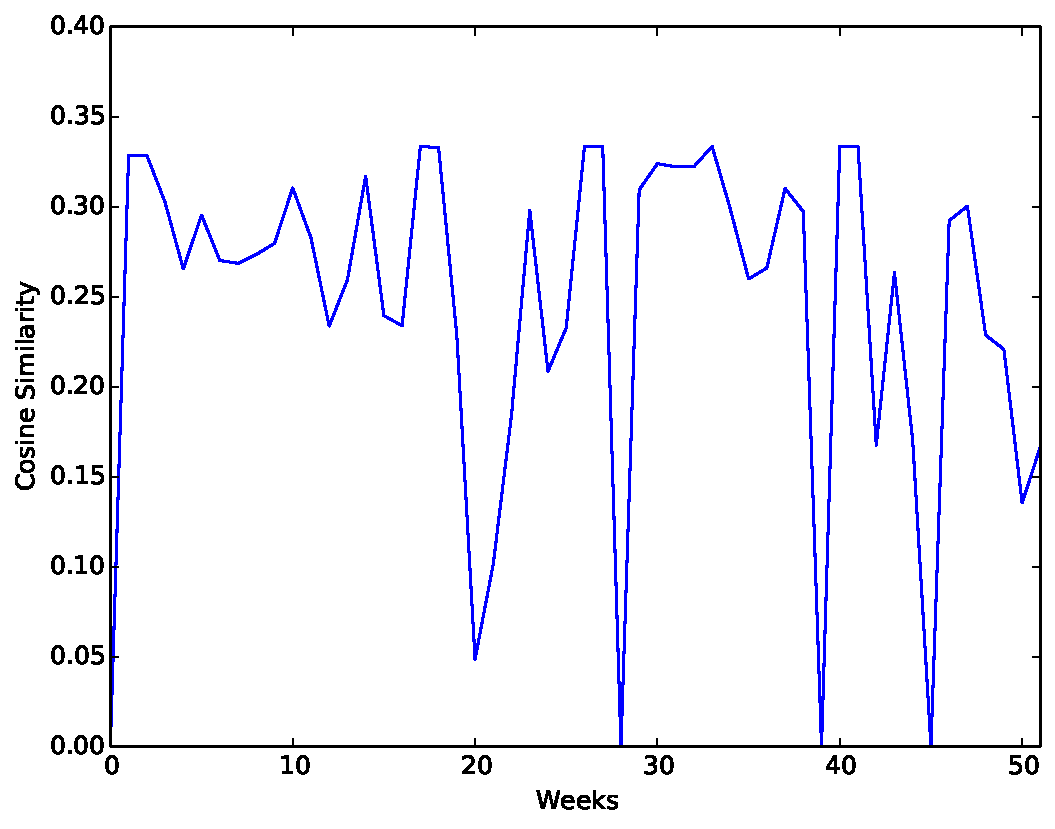
\includegraphics[width=.6\columnwidth]{foo.pdf}
\end{center}
\caption{Provenance graph comparison of climate control system by week.}
\label{figure_climate}
\end{figure}

\section{J1939 Network Bus }

We evaluate Prov-CPS using J1939 CAN data recorded from a Peterbilt truck~\cite{peterbilt}.  This dataset consists of J1939 messages representing normal driving conditions observed on the high speed CAN bus that were logged for a duration of 74 seconds consisting of a total of 16,223 messages.
%
%
%Our experiments calculates the percentage storage savings (i.e., size difference) between the original trace  and the resulting trace file after pruning.
%
%
%\subsection{Target Application: J1939 Network Bus}
The J1939 messaging protocol is an extension of the CAN messaging protocol which is mostly used in heavy-duty trucking vehicles and commercial buses to communicate between in-vehicle electronic control unit (ECUs).  %ECUs are embedded microcontollers contained in vehicles for controlling electrical components. Examples of ECUs are vehicle entertainment systems, engine control module, door control module etc. Each ECU contained in a vehicle listens to messages received on the CAN bus to determine an appropriate message based on the ID parameters. 
A J1939 message consists of a message ID, number of data bytes sent, data, and error checking code. 
%
A J1939 message ID consists of a 29-bit value used to differentiate messages sent by different ECUs. %A message identifier is divided into six categories:  Priority (P), Extended Data Page (EDP), Data Page (DP), PDU format (PF), PDU Specific (PS) and Source Address (SA). SA denotes the origin of the message. 
%An essential component of the message id is the Parameter Group Number (PGN). A PGN is a unique 18 bit identifier used for identifying specific message types. For example the TSC1 messages that determine the engine speed has a PGN value $0000_{16}$. To calculate a PGN number, if the PF value is less than 240, the PGN value can be derived from the combination of the EDP, DP, and PF fields. If the PF field is greater than 240, the PGN field is derived by the combination the P, EDP, DP, PF, and PS components. PGN are further broken down into Suspect Parameter Numbers (SPN) which defines unique data.
For our purposes, we only rely on two fields contained in the message ID: the source address field, which denotes the origin of the message, and the priority field to support priority-based pruning.

From the J1939 dataset, we recreate a trace where each message causes one trace event. We map the source address to the producer identifier in the Prov-CPS model, and map the CAN bus as the controller. The action is a ``receive'' (Rx) activity denoting a passive listener on the bus. We also have the ability to recreate the timestamps from the dataset to be the same in the trace events, but in these experiments we do not use the trace event timestamp. The data object of each trace event consists of the (up to 8) data bytes of the J1939 message. The entire 29-bit message ID is stored as a priority field in the trace event to use for priority-based pruning.

%\subsubsection{\textbf{Malicious Message Injection}} 

Based on the enormous physical constraint that exists in performing real-time message injection attacks on heavy vehicles, and the support of prior work that uses simulation of message injection attacks in CAN networks~\cite{7504089, Otsuka}, we chose to simulate message injection attacks on a CAN bus network. This attack is achieved by recreating the expected log file containing CAN messages received on a CAN bus in an event of a malicious attack. Our message injection attack was modeled after the attacked performed by Mukherjee et al.~\cite{Mukherjee2017APG}. 
%
We simulate message injection attacks by injecting malicious messages into the J1939 dataset using a TSC1 message code, which has a message ID beginning with 21 bits all 0. These messages are used to control the engine's RPM or torque. We inject 10 consecutive TSC1 messages at varied points in the dataset within an existing time gap between two consecutive messages that is greater than 12 times the minimum time gap between two consecutive messages. This is to ensure that we accurately simulate malicious message injection without either time overlap or in excess of the bus bit rate. We chose 10 different log files with the injected attacks in distinctly different regions of the log file (at least 400 messages apart).

For anomaly detection as described in Section~\ref{sec:prov_anomaly}, we take the first quarter of the driving log as a training (observation) set. We do not inject any new messages in this portion of the log, and therefore it is the same in all experiments. The remaining three quarters of the driving log are the test (detection) set, and each anomalous log file contains injected attack messages somewhere in that set. We further divide the training and test sets into equal-sized windows, where the window size is a fraction $f$ of the number of messages in the training set, that is, each window has size equal to $f * n/4$ where $n$ is the number of messages in the log file, i.e., 16,223. A provenance graph is generated for each window, and so the window size is varied as a parameter to explore the effect that scaling graph size has on the performance of the anomaly detector. Performance is measured by collecting the number of true negatives (TN), true positives (TP), false negatives (FN), and false positives (FP) and calculating the true positive rate (TPR) and false positive rate (FPR) in the usual way as:
\[TPR = \frac{TP}{TP+FN}\quad FPR = \frac{FP}{FP+TN}\]
For each window size, i.e., for each different value of $f$, we provide a cumulative TPR and FPR based on the sum of all the positives and negatives recorded over multiple variations of the log file. 


\begin{table*}[tb!] \centering

\caption{Cumulative results of anomaly detection true negative (TN), true positive (TP), false negative (FN), and false positive (FP) for no pruning, FIFO-based pruning, and prioritized pruning based on application priority values.}\label{tab:results}

\begin{tabular}{c|cccc|cccc|cccc}
\textbf{Window Size} & \multicolumn{4}{|c}{\bf No Pruning} & \multicolumn{4}{|c}{\bf FIFO Pruning} & \multicolumn{4}{|c}{\bf Priority Pruning} \\
\textbf{(Messages)} & \textbf{TN} & \textbf{TP} & \textbf{FN} & \textbf{FP} & \textbf{TN} & \textbf{TP} & \textbf{FN} & \textbf{FP} & \textbf{TN} & \textbf{TP} & \textbf{FN} & \textbf{FP}\\ \midrule
15 & 7310 & 13 & 4 & 353 & 7638 & 9 & 8 & 25  & 7607 & 13 & 4 & 56 \\ 
20 & 5609 & 11 & 4 & 376 & 5829 & 8 & 7 & 156  & 5764 & 14 & 1 & 221  \\ 
30 & 3605 & 10 & 3 & 382 & 3788 & 7 & 6 & 199 & 3808 & 9 & 4 & 179 \\ 
40 & 2461 & 12 & 2 & 525  & 2795 & 4 & 10 & 191  & 2658 & 12 & 2 & 328\\ 
50 & 1713 & 9 & 2 & 676 & 2179 & 7 & 4 & 210 & 1971 & 11 & 0 & 418\\ 
126 & 492 & 10 & 0 & 458 & 619 & 5 & 5 & 331 & 591 & 10 & 0 & 359 \\ 
253 & 138 & 11 & 0 & 331 & 201 & 8 & 3 & 268 & 108 & 11 & 0 & 361 \\ 
506 & 9 & 11 & 0 & 220  & 25 & 10 & 1 & 204 & 0 & 11 & 0 & 229 \\ 
1013 & 9 & 11 & 0 & 100 & 0 & 11 & 0 & 109 & 0 & 11 & 0 & 109 \\
\end{tabular}

\end{table*}

%\begin{table*}[] \centering
%%\ra{1.3}
%
%\begin{tabular}{@{}llllr@{}}\toprule
%\textbf{F} & \textbf{True Negative} & \textbf{True Positive} & \textbf{False Negative} & \textbf{False Positive}\\ \midrule
%\textbf{0.00391} & 7638 & 9 & 8 & 25 \\ \hdashline
%\textbf{0.00500} & 5829 & 8 & 7 & 156 \\ \hline
%\textbf{0.00750} & 3788 & 7 & 6 & 199 \\ \hline
%\textbf{0.0100} & 2795 & 4 & 10 & 191 \\  \hline
%\textbf{0.0125} & 2179 & 7 & 4 & 210 \\ \hline
%\textbf{0.0313} & 619 & 5 & 5 & 331 \\ \hline
%\textbf{0.0625} & 201 & 8 & 3 & 268 \\ \hline
%\textbf{0.125} & 25 & 10 & 1 & 204 \\ \hline
%\textbf{0.250} & 0 & 11 & 0 & 109 \\  \midrule
%
%\bottomrule
%\end{tabular}
%
%\caption{Experimental Results of TP, TN, FP, and FN rates without pruning with FIFO pruning}
%\end{table*}
%
%\begin{table*}[] \centering
%%\ra{1.3}
%
%\begin{tabular}{@{}llllr@{}}\toprule
%\textbf{F} & \textbf{True Negative} & \textbf{True Positive} & \textbf{False Negative} & \textbf{False Positive}\\ \midrule
%\textbf{0.00391} & 7634 & 3 & 14 & 29 \\ \hdashline
%\textbf{0.00500} & 5853 & 4 & 11 & 132 \\ \hdashline
%\textbf{0.00750} & 3974 & 2 & 11 & 13 \\ \hdashline
%\textbf{0.0100} & 2919 & 3 & 11 & 67 \\  \hdashline
%\textbf{0.0125} & 2319 & 4 & 7 & 70 \\ \hdashline
%\textbf{0.0313} & 735 & 2 & 8 & 215 \\ \hdashline
%\textbf{0.0625} & 337 & 2 & 9 & 132 \\ \hdashline
%\textbf{0.125} & 160 & 1 & 10 & 69 \\ \hdashline
%\textbf{0.250} & 54 & 1 & 10 & 55 \\  \midrule
%
%\bottomrule
%\end{tabular}
%
%\caption{Experimental Results of TP, TN, FP, and FN rates without pruning with Priority pruning}

%\end{table*}

%\begin{figure*}[!htb]
%   \begin{minipage}{0.48\textwidth}
%     \centering
%     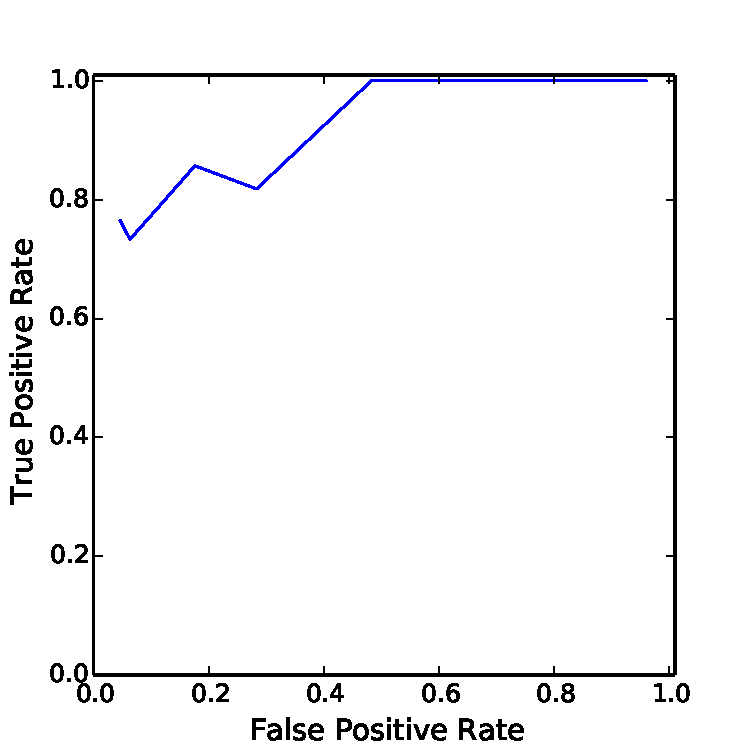
\includegraphics[width=.7\linewidth]{roc_curve_0.pdf}
%     \caption{Interpolation for Data 1}\label{Fig:ROC without Pruning}
%   \end{minipage}\hfill
%   \begin {minipage}{0.48\textwidth}
%     \centering
%     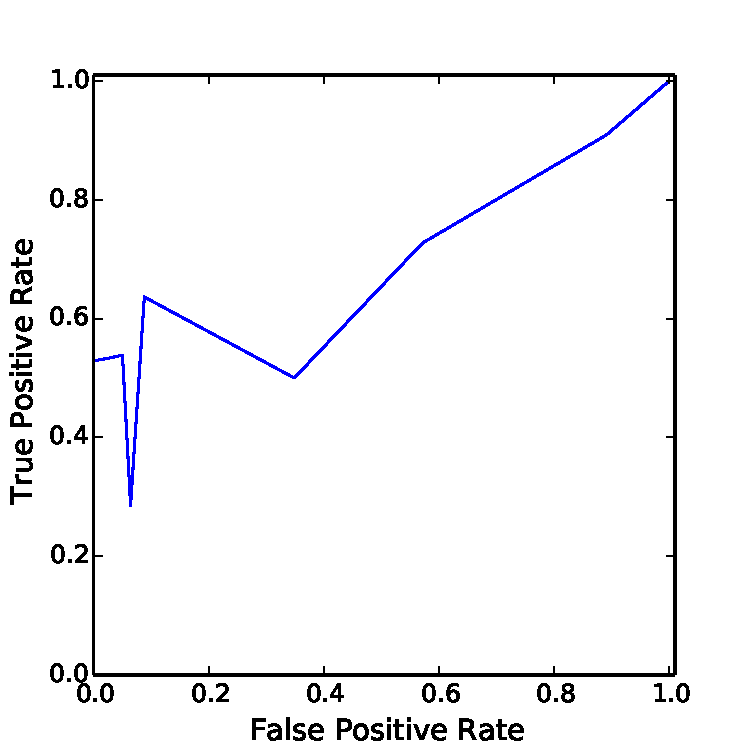
\includegraphics[width=.7\linewidth]{roc_curve_1.pdf}
%     \caption{Interpolation for Data 2}\label{ROC with Pruning}
%   \end{minipage}
%\end{figure*}


\begin{figure*}[!htb]
 
\centering
\subfloat[ROC with No Pruning]{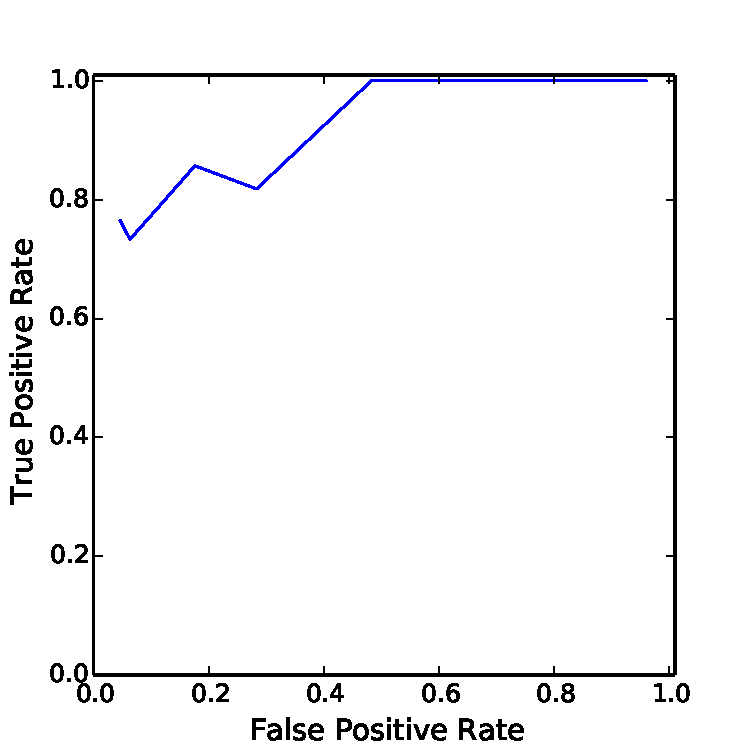
\includegraphics[width=.3\textwidth]{roc_curve_0.pdf}\label{fig:roc_curve_0}}
\hfill
\subfloat[ROC with FIFO Pruning]{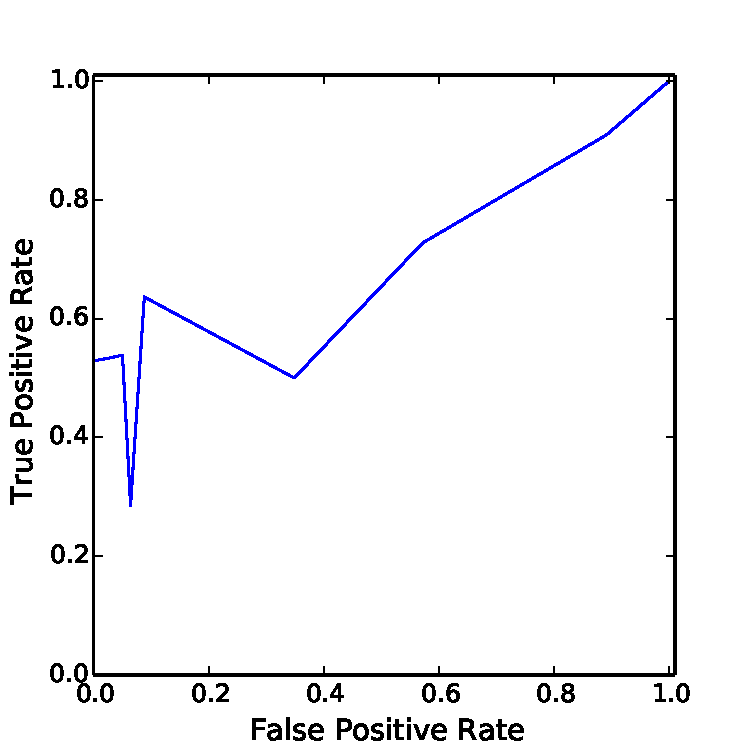
\includegraphics[width=.3\textwidth]{roc_curve_1.pdf}\label{fig:roc_curve_1}}
\hfill
\subfloat[ROC with Priority Pruning]{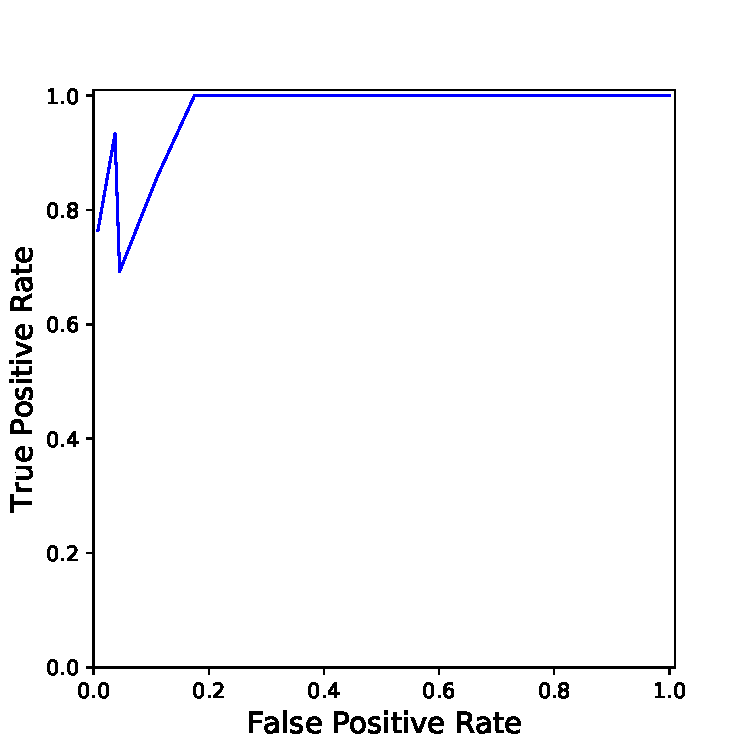
\includegraphics[width=.3\textwidth]{roc_curve_2.pdf}\label{fig:roc_curve_2}}
\caption{Receiver operating characteristic (ROC) curves without pruning and with FIFO or Priority pruning.}
\label{fig:roc}

\end{figure*}


Table~\ref{tab:results} shows the cumulative results of anomaly detection summed over 10 log files each containing 1 set of 10 injected messages. Each approach to pruning---no pruning, FIFO pruning, and priority pruning---was evaluated using the same input log files.  For the pruning algorithms, we chose to prune one-half of the window size for these experiments. Each row shows a different window size, which corresponds to a different value of $f$ ranging between 0.0039 to 0.25 with corresponding window sizes between 15 and 1013 messages. Cumulative results also are presented using a receiver operating characteristic (ROC) curve showing how performance changes with $f$. The ROC curve is a widely used metric for evaluating IDS systems. It is generated by plotting the TPR over the FPR. Figure~\ref{fig:roc} shows the ROC curve for each pruning algorithm (no pruning, FIFO pruning, and priority-based pruning) separately evaluated in the same way using the same modified datasets. As $f$ increases, the window sizes get larger and so do the graphs, which increases their relative variability and therefore decreases the similarity scores, thus resulting in higher TPR and FPR. With smaller $f$ and therefore small graphs, the anomaly detection algorithm is better able to match the features of graphs in the training and testing sets, so TPR can stay high while FPR decreases; note that with smaller window sizes, there are also more decisions (positives and negatives) to make. 


\section{Summary}
This chapter evaluates the effectiveness of PROV-CPS using an anomaly detection algorithm as described in chapter 6. The anomaly detection algorithm is evaluated on a climate control system and a J1939 network. In the climate control system, we compared the temperature values generated by preceding weeks. Preliminary result indicates the detection of anomalous irregularities in temperature data. On the J1939 network, we evaluated false positive and true positive rates based on a defined window size ($f$ value) using a dataset which consists of malicious J1939 messages. The result indicates that the smaller the window size, the better the accuracy of detecting anomalous instances that exists in the dataset.
         % Chapter 6
% chap7.tex (Bogus chapter)

\chapter{Extra Chapter}

This is an extra chapter added into Patrick's thesis to illustrate
the use of figures and tables and the inclusion of a pdf file.

First the tables are shown as Table~\ref{smalltable} and
Table~\ref{smalltable2}. Then the
figure is shown in Figure~\ref{autom}.

\begin{table}
\begin{center}
\caption[A long caption]{A long caption.
In this table example, we have a very
long caption that does not fit on one line. The text of the
caption should line up on the left. The text inside the square
brackets will be included in the List of Tables.}
\label{smalltable}
\vspace{0.2in}
\begin{tabular}{|c|c|c|}\hline
2 & 3 & 300 \\ \hline
3 & 4 & 400 \\ \hline
4 & 5 & 500 \\ \hline
5 & 6 & 600 \\ \hline
\end{tabular}
\end{center}
\end{table}

\begin{table}
\begin{center}
\caption{Example of a table}
\label{smalltable2}
\vspace{0.2in}
\begin{tabular}{|c|c|c|}\hline
2 & 3 & 300 \\ \hline
3 & 4 & 400 \\ \hline
4 & 5 & 500 \\ \hline
5 & 6 & 600 \\ \hline
\end{tabular}
\end{center}
\end{table}

\begin{figure}
\begin{center}
\resizebox{\textwidth}{!}
  {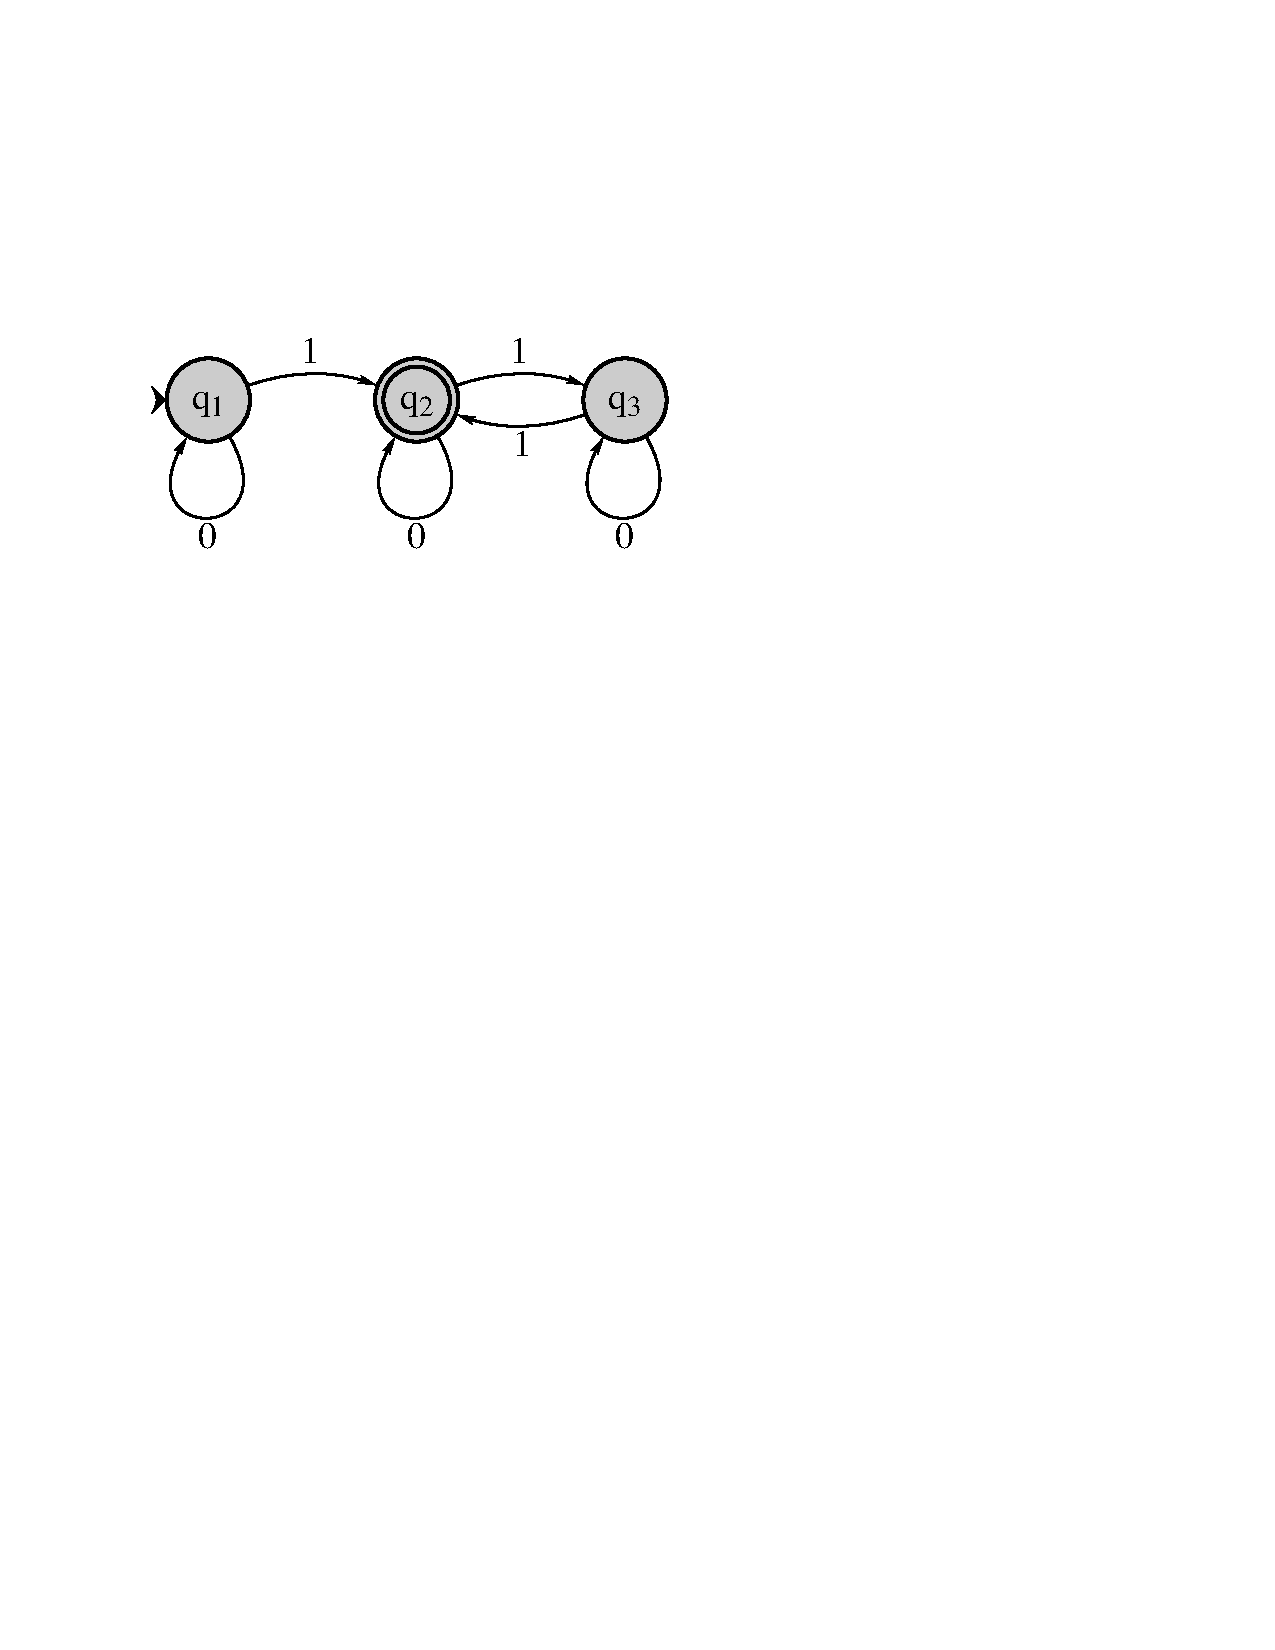
\includegraphics{automin1.pdf}}
\end{center}
\caption{A simple finite automaton}
\label{autom}
\end{figure}
         % Chapter 7, chap7.tex contains an
                        % example of figs and tables and inclusion of pdf.

%%%%%%%%%%%%%%%%%%%%
% Concluding Pages %
%%%%%%%%%%%%%%%%%%%%%%%%%%%%%%%%%%%%%%%%%%%%%%%%%%%%%%%%%%%%%%%%%%%%%%%%%%%%%%%%

% Bibliography or References, REQUIRED

% If using bibtex, create or modify the refs.bib file
% and use (uncomment) the following three lines.
\bibliographystyle{plain}     
%\bibliographystyle{alpha}
\addcontentsline{toc}{chapter}{\bibname}
\bibliography{refrences}         

% If using the ``thereference'' environment instead, modify the ref.tex file
% and use the following line
%% ref.tex {References}

\addcontentsline{toc}{chapter}{References}
\begin{thereferences}{99}

\bibitem{Cook1971}
S.~Cook,
 ``The complexity of theorem-proving procedures,''
 {\it Proceedings of the 3rd ACM Symposium on Theory of Computing},
 Shaker Heights, Ohio, 1971, pp.~151--158.

\bibitem{Garey1979}
M.~R.~Garey and D.~S.~Johnson,
 {\it Computers and Intractability: A Guide to the Theory of\/
 {\rm NP}-Completeness},
 W.~H.~Freeman, San Francisco, 1979.

\bibitem{Karp1972}
R.~Karp,
 ``Reducibility among combinatorial problems,''
 in: R.~Miller and J.~Thatcher (eds.),
 {\it Complexity of Computer Computations},
 Plenum Press, New York, 1972, pp.~85--103.

\bibitem{Kearfott1996}
R.~B.~Kearfott and V.~Kreinovich (eds.),
 {\it Applications of Interval Computations},
 Kluwer Academic Publishers, Norwell, MA, 1996.

\bibitem{Kreinovich1993}
V.~Kreinovich, A.~V.~Lakeyev and S.~I.~Noskov,
 ``Optimal solution of interval linear systems is intractable (NP-hard),''
 {\it Interval Computations},
 1993, No. 1, pp. 6--14.

\bibitem{Kreinovich1996a}
 V.~Kreinovich, A.~V.~Lakeyev and J.~Rohn ,
 ``Computational complexity of interval algebraic problems: some are feasible
 and some are computationally intractable: a survey,''
 in: G.~Alefeld and A.~Frommer (eds.),
 {\it Scientific Computing and Validated Numerics},
 Akademie-Verlag, Berlin, 1996, pp.~293--306.

\bibitem{Kreinovich1996b}
 V.~Kreinovich, A.~V.~Lakeyev, J.~Rohn and P.~Kahl,
 {\it Feasible? Intractable? On Computational Complexity of Data Processing
 and Interval Computations},
 Kluwer Academic Publishers, Norwell, MA, 1996 (to appear).

\bibitem{Kulisch1981}
U.~Kulisch and W.~L.~Miranker,
 {\it Computer Arithmetic in Theory and Practice},
 Academic Press, NY, 1981.

\bibitem{Lakeyev1995}
A.~V.~Lakeyev and V.~Kreinovich,
 ``If input intervals are small enough, then interval computations are almost
 always easy,''
 {\it Reliable Computing},
 Supplement (Extended Abstracts of APIC'95: International Workshop on 
 Applications of Interval Computations),
 1995, pp. 134--139.

\bibitem{Levin1973}
L.~Levin,
 ``Universal sequential search problems,''
 {\it Problems of Information Transmission},
 1973, Vol. 9, No. 3, pp. 265--266.

\bibitem{Moore1959}
R.~E.~Moore,
 ``Automatic error analysis in digital computation,''
 {\it Technical Report LMSD-48421},
 Lockheed Missiles and Space Co., Palo Alto, CA, January 1959.

\bibitem{Moore1966}
R.~E.~Moore,
 {\it Interval Analysis},
 Prentice Hall, Englewood Cliffs, NJ, 1966.

\bibitem{Neumaier1990}
A.~Neumaier,
 {\it Interval Methods for Systems of Equations},
 Cambridge University Press, Cambridge, 1990.

\bibitem{Rabinovich1995}
S.~G.~Rabinovich,
 {\it Measurement Errors: Theory and Practice},
 American Institute of Physics, NY, 1995.

\end{thereferences}


% If including appendices, uncomment the following lines,
% adding more includes if needed.
%\StartAppendix
%\include{AppendixA}         % Example of how to include an appendix

%% vitae.tex (Curriculum Vitae)

\addcontentsline{toc}{chapter}{Curriculum Vitae}
\chapter*{Curriculum Vitae}

Patrick Thor Kahl was born on July 12, 1961. The first son of Ulf Thor Gustav 
Kahl and Carolyn Kahl, he graduated from Coronado High School, El Paso, Texas, 
in the spring of 1979.  He entered Auburn University in the fall of 1979, and,
in the spring of 1982, The University of Texas at El Paso.  In 1985 he joined
the United States Navy where he served for eight years, most of it aboard the
submarine USS Narwhal (SSN671).  In the fall of 1993, after being honorably
discharged from the navy, Patrick resumed his studies at The University of
Texas at El Paso.  While pursuing his bachelor's degree in Computer Science he
worked as a Teaching Assistant, and as a programmer at the National
Solar Observatory at Sunspot, New Mexico.  He received his bachelor's degree
in Computer Science in the summer of 1994.

In the fall of 1994, he entered the Graduate School of The University of Texas 
at El Paso.  While pursuing a master's degree in Computer Science he worked as 
a Teaching and Research Assistant, and as the Laboratory Instructor for the
1995 Real-Time Programming Seminar at the University of Puerto Rico,
Mayag\"{u}ez Campus.  He was a member of the Knowledge Representation Group
and the Rio Grande Chapter of the Association for Computing Machinery.

\medskip

\noindent
Permanent address: 6216 Sylvania Way

\noindent
\hspace{1.42in}
El Paso, Texas 79912-4927

\vfill

% The following is no longer needed when typed by the author.
%\noindent
%This thesis was typed by <name of typist>.


         % Curriculum Vitae      REQUIRED

%%%%%%%%%%%%%%%%%%%%%%%%%%%%%%%%%%%%%%%%%%%%%%%%%%%%%%%%%%%%%%%%%%%%%%%%%%%%%%%%

\end{document}
